\documentclass[11pt]{beamer}
\usetheme{Madrid}
\usepackage[spanish]{babel}
\usepackage{amsmath}
\usepackage{amsfonts}
\usepackage[utf8]{inputenc}
\usepackage{amssymb}
\usepackage{graphicx}

\title[Tipos dependientes y Agda]{Introducción a los tipos dependientes y a la programación verificada en Agda}
\author{Marcelo Lynch}

\setbeamersize{text margin left=10mm, text margin right=12mm} 

\newcommand{\bit}{\begin{itemize}\setlength\itemsep{1em}}
\newcommand{\biti}{\begin{itemize}\setlength\itemsep{0.3em}}
\newcommand{\eit}{\end{itemize}}

%\setbeamercovered{transparent} 
%\setbeamertemplate{navigation symbols}{} 

%gets rid of footer
%will override 'frame number' instruction above
%comment out to revert to previous/default definitions
%\setbeamertemplate{footline}{}

%\logo{} 
\institute[ITBA]{Instituto Tecnológico de Buenos Aires} 
%\date{} 
%\subject{} 
\begin{document}

\begin{frame}
\titlepage
\end{frame}

%\begin{frame}
%\tableofcontents
%\end{frame}

\begin{frame}{Programación verificada}
\begin{itemize}
\item Se está volviendo cada vez más importante garantizar que el software \textit{hace lo que queremos que haga}.
\item[]
\item Los \textit{bugs} pueden ser muy costosos y hasta costar vidas 
\item[]
\item \textbf{Objetivo}: que nuestros programas y algoritmos sean \textit{correctos} de acuerdo a alguna \textit{especificación}
\end{itemize}
\end{frame}

\begin{frame}{Técnicas de verificación}
Existen varias maneras de aproximarse a este objetivo: \\

\begin{itemize}
\setlength\itemsep{1em}
\item[]
\item Testing y revisión de pares
%\pause
\item Análisis estático y dinámico para encontrar bugs
%\pause
\item Verificación formal
\begin{itemize}
\item Model checking
\item Verificación deductiva: demostradores de teoremas
\end{itemize}
\end{itemize}
\end{frame}

\begin{frame}{Verificación formal}
\bit 
\setlength\itemsep{1em}
\item Los \textbf{métodos formales} nos permiten \textbf{demostrar la corrección con rigor matemático}. 

\item Podemos describir a los métodos formales como ``la matemática aplicada para modelar y analizar sistemas de software''.

\item Esta verificación se hace proveyendo una demostración formal de un modelo matemático del sistema.
\bit
\item La correspondencia entre el modelo matemático y el sistema real se presume.
\eit
\eit

\end{frame}

\begin{frame}{Demostradores de teoremas}
El nivel de automaticidad de estas herramientas nos deja categorizarlas en:

\bit
\item[]
\item Demostradores automáticos
\item Asistentes de demostraciones
\item Verificadores de demostraciones
\eit
\end{frame}

\begin{frame}{Asistentes de demostraciones}
\bit
\setlength\itemsep{1em}
\item Incluyen una interfaz en la que el usuario guía de alguna manera la búsqueda de la demostración
\item Se habla en estos casos de una ``colaboración humano-máquina''
\item Ejemplos notables:
\biti
\item Coq
\item Isabelle
\item Agda 
\eit
\eit
\end{frame}

\begin{frame}{Agda - Introducción}
\bit
\item Agda es un lenguaje funcional con \textit{tipos dependientes}, y sintaxis similar a Haskell
\item Al mismo tiempo es un asistente de demostraciones que funciona dentro del mismo lenguaje (mediante su type checker)
\item Desarrollado mayormente por Ulf Norell para su tesis de doctorado en la Universidad Tecnológica Chalmers en Gotemburgo, Suecia
\eit
\end{frame}

\begin{frame}{Agda y Haskell}
\bit
\item Agda está desarrollado en Haskell
\item La sintaxis de Agda esta inspirada en Haskell y el estilo de programación es similar
\item Tienen distintas teorías subyacentes
\biti
\item Haskell está basado en System F (lambda cálculo tipado con polimorfismo paramétrico)
\item Agda está basado en la teoría de tipos dependientes de Martin-Löf
\eit
\item Agda posee un \textbf{termination checker}: todos los programas deben terminar. Es decir, no hay recursión general y no es Turing-completo.  
\eit
\end{frame}

\begin{frame}{Teorías de tipos}
\bit
\item Se llama \textbf{teoría de tipos} a una serie de sistemas formales que sirven como alternativa a la teoría de conjuntos como fundamento formal de la matemática. 
\item Los matemáticos y científicos de la computación trabajan siempre con \textit{construcciones} u \textit{objetos} teóricos. 
\item Implícitamente se suele categorizar a los objetos con los que trabaja, asociándolos a un \textit{tipo}. 
\item Las teorías de tipos hacen explícita esta asociación, tratando a los distintos tipos como ``ciudadanos de primera clase''
\eit
\end{frame}

\begin{frame}{La teoría de tipos de Martin-Löf}
\bit
\item Presentada por Per Martin-Löf como un fundamento matemático intuicionista (constructivista): por esto es también conocida como \textit{teoría de tipos intuicionista}. 
\item La descripción de la teoría y sus elementos se hace a partir de \textit{juicios}, es decir afirmaciones en el lenguaje metalógico (por afuera del sistema)
\biti 
\item Así, por ejemplo, en lugar de \textit{definir} el concepto de tipo veremos en qué condiciones se puede decir (es decir, emitir un juicio, o ``explicar'') que algo \textit{es un tipo}.
\eit
\eit
\end{frame}

\begin{frame}{Tipos}
Podemos emitir el juicio ``$A$ \textbf{es un tipo}'' cuando conocemos:
\bit
\item[]
\item Cuándo un objeto pertence al tipo (las condiciones de pertenencia)
\item que significa que dos objetos del tipo sean iguales (mediante una relación de equivalencia)
\eit
\end{frame}
\begin{frame}{Tipos}
\bit
\item La pertenencia de un objeto $a$ al tipo $A$ se nota 
$a \in A$ o $a : A$.
\item Decimos que $B$ es una \textit{familia de tipos} indexada por $A$ si $B$ es una asignación que para cada $a \in A$ asigna un tipo $B(a)$. 
\eit
\end{frame}

\begin{frame}{Términos y objetos}
\bit
\item La teoría tiene asociada una noción de cómputo, que es relevante al contextualizarla dentro de un lenguaje de programación
\item En rigor en lugar de objetos hablamos de \textbf{términos}
\biti
\item Por ejemplo, $4$, $2 + 2$ y $2 \cdot 2$ podrían ser términos distintos del tipo \textbf{Nat}
\eit
\pause
\item Existen \textbf{reglas de reescritura} sobre los términos:
\biti
\item Por ejemplo, $2 + 2$ se puede reescribir mediante una serie de reglas de reescritura al término $4$
\item Decimos que $2 + 2$ \textit{reduce a} $4$
\item Podemos pensar a dos términos que se pueden reducir a un mismo término como ``iguales'' en cierto sentido: esta noción se llama \textit{igualdad definicional}
\eit
\eit
\end{frame}

\begin{frame}{Ejemplos de tipos: \textbf{Set}}
\bit
\item La colección de todos los conjuntos forma un tipo, que podemos llamar \textbf{Set}.
\item También podemos pensar al tipo \textit{\textbf{Set}} como un tipo que contiene a otros tipos (pensando a los tipos estructuralmente como conjuntos de objetos). Esta es la noción que usamos en Agda, donde si $A$ es un tipo entonces $A : Set$.
\pause
\biti
\item Observación: $Set$ es un tipo, pero el juicio $Set : Set$, lleva a la clásica inconsistencia de Bertrand Russell.
\item Esto se puede arreglar introduciendo una jerarquía de tipos $Set_0$, $Set_1$, $...$, con \textbf{Set} = $Set_0$ y $Set_{i} : Set_{i+1}$. No nos adentraremos demasiado en esto, y manejamos a continuación tipos de ``primer nivel" que estan en \textbf{Set}.
\eit
\eit
\end{frame}

\begin{frame}{Tipos funcionales}
\bit
\item Si $A$ y $B$ son tipos podemos introducir el tipo $A \rightarrow B$, el espacio de funciones de $A$ a $B$.
\item Un elemento $f \in A \rightarrow B$ se puede \textit{aplicar} a cualquier $a \in A$, y tenemos $f(b) \in B$.
\eit
\end{frame}


\begin{frame}{Pares ordenados}
\bit

\item Si $A$ y $B$ son tipos podemos introducir el tipo $A \times B$ de pares ordenados: la primera componente tiene elementos de $A$ y la segunda elementos de $B$.
\item Notamos a un elemento de $A \times B$ como $(a,b)$.
\item Los tipos de pares ordenados vienen equipados con proyecciones $\pi_1, \pi_2$ funciones tales que $\pi_1 ((a,b)) = a$ y $\pi_2 ((a,b)) = b$.
\eit
\end{frame}

\begin{frame}{El tipo suma}
\bit
\item Si $A$ y $B$ son tipos podemos introducir el tipo $A + B$, la suma disjunta de $A$ y $B$. 
\item Un elemento de este tipo será o bien un elemento de $A$ o uno de $B$, junto con una indicación de si provino de $A$ o de $B$
\item Todos los elementos de $A + B$ pueden describirse mediante dos funciones $inj_A : A \rightarrow A + B$ e $inj_B : B \rightarrow A + B$. 
\item En Haskell el concepto análogo es el the la forma del tipo \texttt{Either a b = Left a | Right b}, donde podemos saber el ``origen'' por pattern matching en los constructores \texttt{Left} y \texttt{Right} (estos constructores son análogos a las funciones $inj$). 
\eit
\end{frame}

\begin{frame}{Tipos dependientes}
\bit
\item El concepto central de esta teoría de tipos es el de \textbf{tipo dependiente}
\item La definición de un tipo dependiente \textit{depende de un valor} (y no de otros tipos como lo que veníamos viendo).
\item Veremos que la existencia de tipos dependientes es lo que nos deja hacer demostraciones usando esta teoría de tipos
\eit
\end{frame}


\begin{frame}{Funciones dependientes}
Si $B$ es una familia de tipos sobre $A$, existe el llamado producto dependiente, tipo de funciones dependientes o \textit{tipo pi}:
\[ \prod_{a\in A}B(a)
    \]

Este tipo contiene funciones con dominio (o entrada) en $A$ pero cuyo codominio (o tipo de salida) depende del valor en la que se aplica la función. 

\end{frame}

\begin{frame}{Funciones dependientes (tipos $\Pi$)}
Por ejemplo: si llamamos $VecN(n)$ al conjunto de listas de $n$ elementos naturales, podemos considerar una función $f$ que aplicada en un numero natural $n$ resulta en una lista de $n$ ceros. Con esto:
 
\[
  f \in \prod_{n \in \mathbb{N}} VecN(n)
\]

Notemos que cuando $B$ es una asignación constante, este tipo corresponde al tipo de funciones $A \rightarrow B$ antes mencionado (donde el codominio no depende del valor de entrada).
\end{frame}

\begin{frame}{Pares dependientes (tipos $\Sigma$)}
Los elementos de los tipos $\Sigma$ son pares ordenados donde el tipo de la segunda componente depende del valor en la primera componente.\\

Esto es, si $B$ es una familia de tipos sobre $A$, existe el tipo de pares dependientes: \[ \sum_{a \in A} B(a) \]

Cuando $B$ es una asignación constante, este tipo corresponde al tipo de pares ordenados $A \times B$.
\end{frame}


\begin{frame}{El tipo igualdad}
\bit
\item Dados dos términos $x$, $y$ puede introducirse el tipo igualdad $x \equiv y$. 

\item Existe un único constructor \texttt{refl} para cada tipo $A$ que dado un objeto de $A$ devuelve un valor de $a \equiv a$:
\eit
\[
  \texttt{refl} \in \prod_{a \in A} a \equiv a
\]

\end{frame}


\begin{frame}{El tipo igualdad}

\bit

\item Notemos que $\texttt{refl}$ es la única forma de construir (encontrar, describir) un valor del tipo igualdad
\item Esto significa que si bien podemos hablar de un tipo $x \equiv y$ para cualesquiera dos términos $x$, $y$, el tipo $x \equiv y$ solo estará habitado si $x$ es igual a $y$.
\eit
\end{frame}

\begin{frame}{¿El tipo igualdad?}
 Con la introducción del tipo igualdad nos acercamos a la idea central que nos permite demostrar cosas en lenguajes como Agda: estamos diciendo que existe un \textbf{tipo} que representa a la \textbf{igualdad}, que es una afirmación lógica.
\bit
\item[]
\eit
Veremos ahora precisamente como se establece este paralelismo entre tipos y fórmulas lógicas

\end{frame}

\begin{frame}{Lógica intuicionista}
\bit
\item En la lógica clásica vale el principio del tercero excluido: ``o bien $A$ es verdadero, o bien $A$ es falso''.

\item La lógica intuicionista rechaza el principio del tercero excluido: exige una demostración concreta o bien de que $A$ es verdadero o de que $B$ es verdadero para concluir que $A \vee B$ es verdadero: en otras palabras, con la demostración de $A \vee B$ debemos saber \textit{cuál de los dos vale}.

\item La lógica intuicionista es \textit{constructivista}: para demostrar la existencia de un elemento que satisface una propiedad hay que construirlo, exhibirlo.
\eit

\end{frame}

\begin{frame}{Proposiciones como tipos}
El concepto de \textit{proposiciones como tipos}, o \textit{correspondencia de Curry-Howard} es la relación directa que existe entre las fórmulas de la lógica (proposiciones) con los tipos en la teoría de tipos. 

\begin{table}[ht]
    \centering
    \begin{tabular}{|c|c|}
    \hline
    \textit{\textbf{Lógica}} & \textit{\textbf{Teoría de tipos}} \\ \hline
    Proposición, fórmula     & Tipo                              \\ \hline
    Demostración             & Programa                          \\ \hline
    Evidencia                & Habitante de un tipo              \\ \hline
    \end{tabular}
    \caption{Correspondencia de Curry-Howard}
    \label{tab:cwi}
    \end{table}


\end{frame}

\begin{frame}{Proposiciones como tipos}
Aquí ya vemos como la correspondencia se da en el marco de la lógica intuicionista:
\bit
\item[]
\item La \textit{evidencia} la da un habitante concreto de un tipo
\item Una demostración se da con un \textit{programa}, que es una \textbf{verdadera construcción de la evidencia} 
\eit
\end{frame}

\begin{frame}{La correspondencia de Curry-Howard}
\bit
\item $A \land B$ corresponde a $A \times B$
\item $A \vee B$ corresponde a $A + B$
\item $A \Rightarrow B$ corresponde a $A \rightarrow B$
\item $\forall x:A.\ B(x)$ corresponde a $\prod_{x\in A} B(x)$
\item $\exists x:A.\ B(x)$ corresponde a $\sum_{x\in A} B(x)$
\eit

\end{frame}

\begin{frame}{Demostrando con el sistema de tipos}

Podemos imaginar ahora cómo se demuestran las propiedades de los programas en un lenguaje con tipos dependientes como Agda: \textbf{simplemente debemos exhibir un elemento que habite el tipo que corresponde a la proposición que queremos demostrar}. 

\bit
\item[]
\eit

Es decir, para demostrar una propiedad como \[ \forall n : \mathbb{N}\ .\ \forall m : \mathbb{N}\ .\ n + m = m + n  \] basta con exhibir (construir) un elemento del tipo \[ \prod_{n \in \mathbb{N}}\prod_{m \in \mathbb{N}} n + m \equiv m + n \]
\end{frame}

\begin{frame}{Programando en Agda - Definiciones}
\begin{figure}
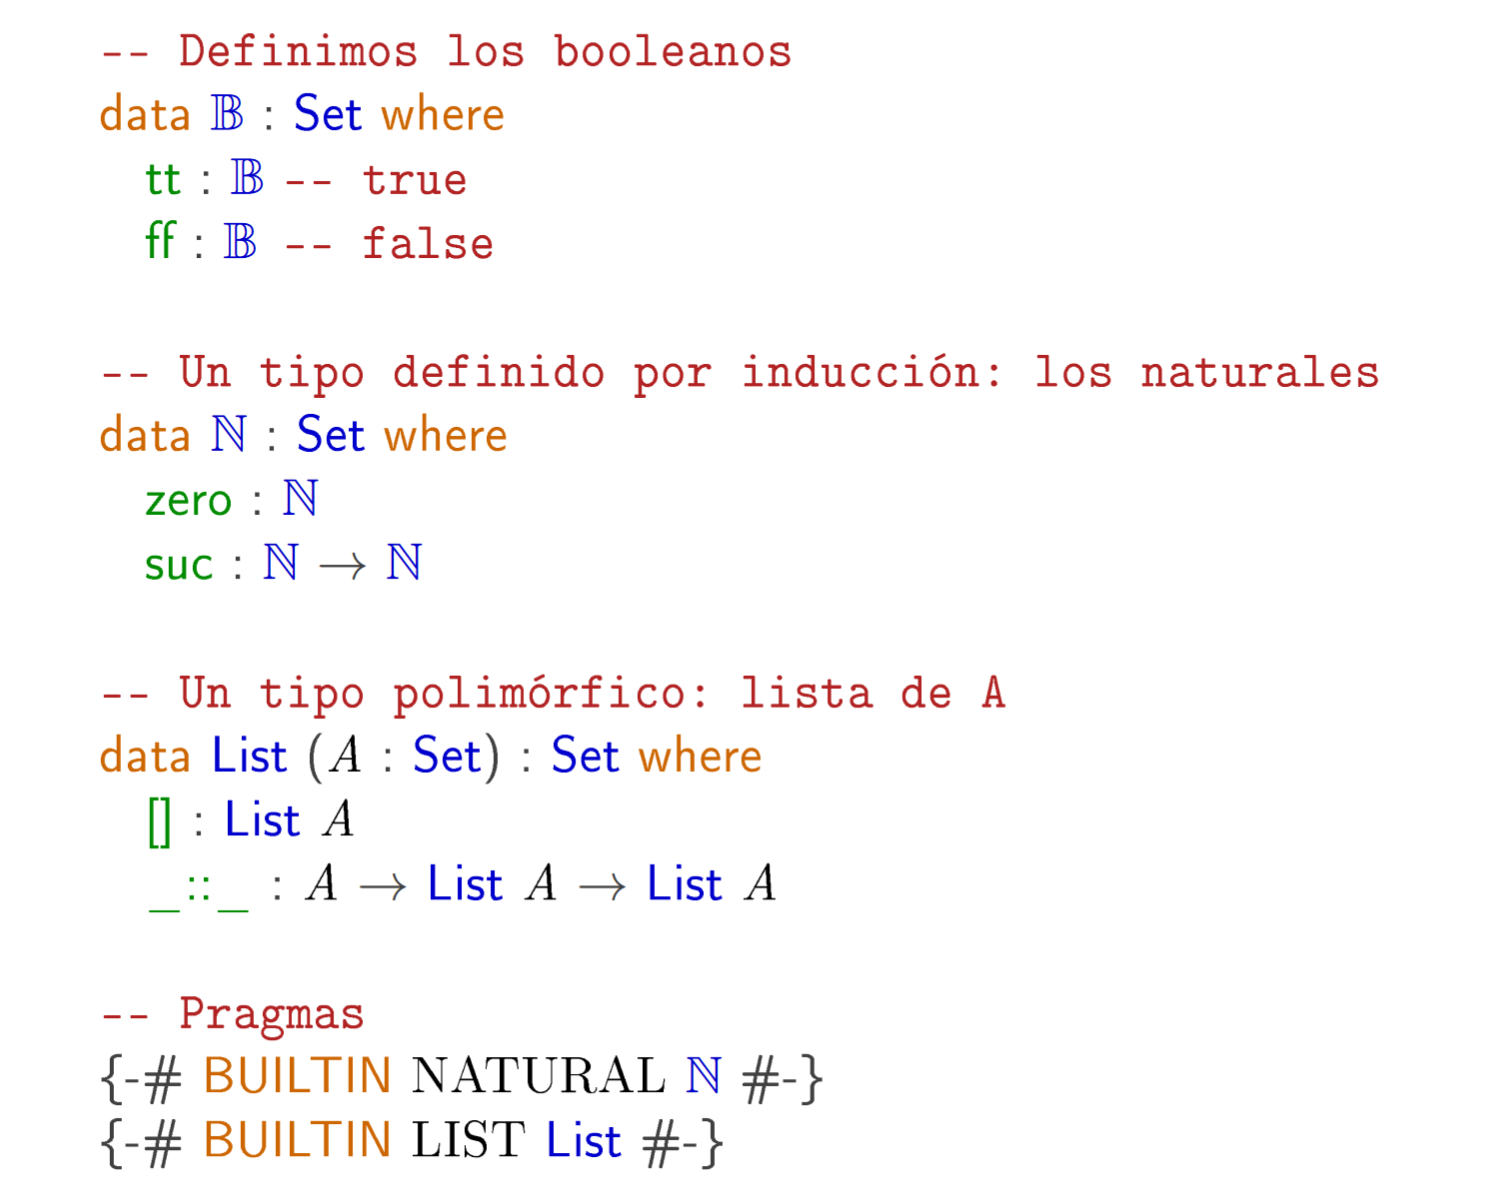
\includegraphics[scale=0.5]{img/defs}
\end{figure}\end{frame}

\begin{frame}{Funciones}
\begin{figure}
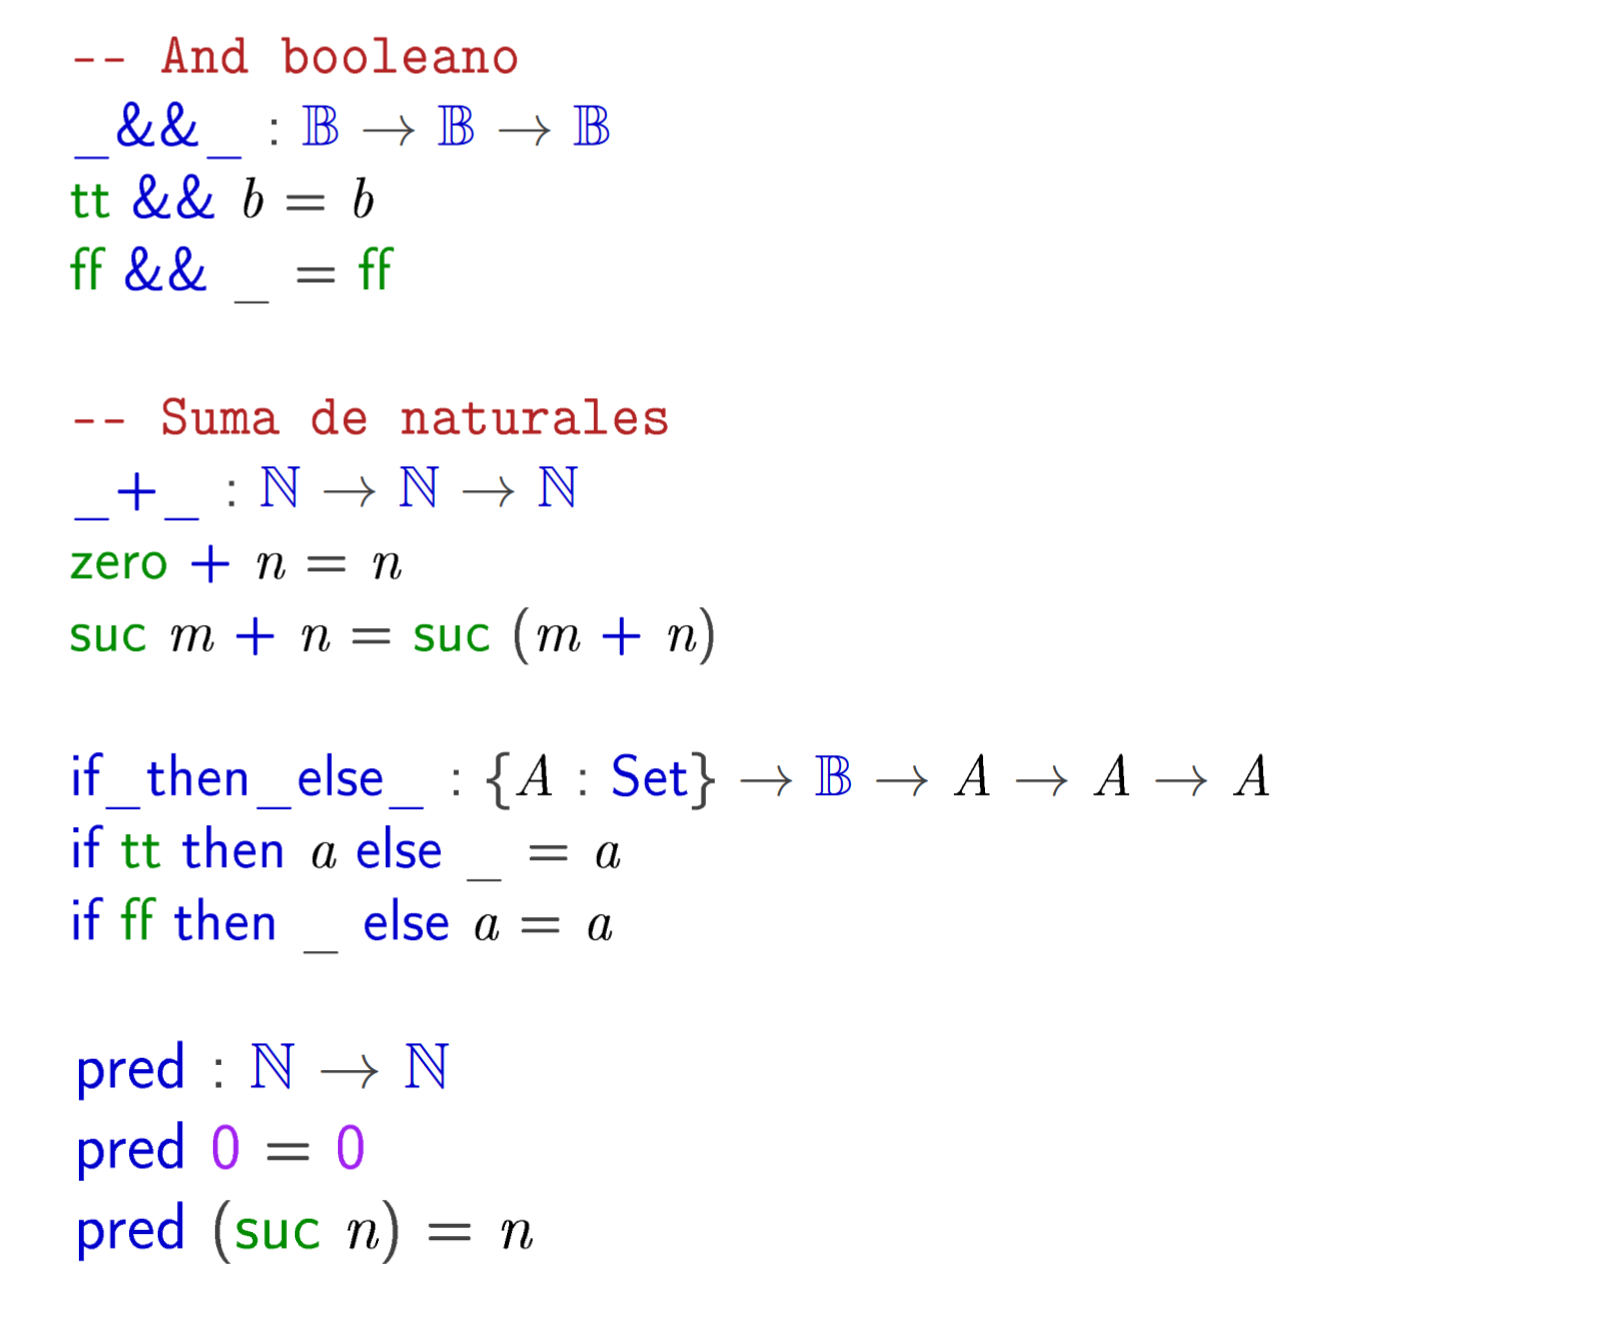
\includegraphics[scale=0.4]{img/funcs}
\end{figure}\end{frame}


\begin{frame}{Tipos dependientes}
\begin{figure}
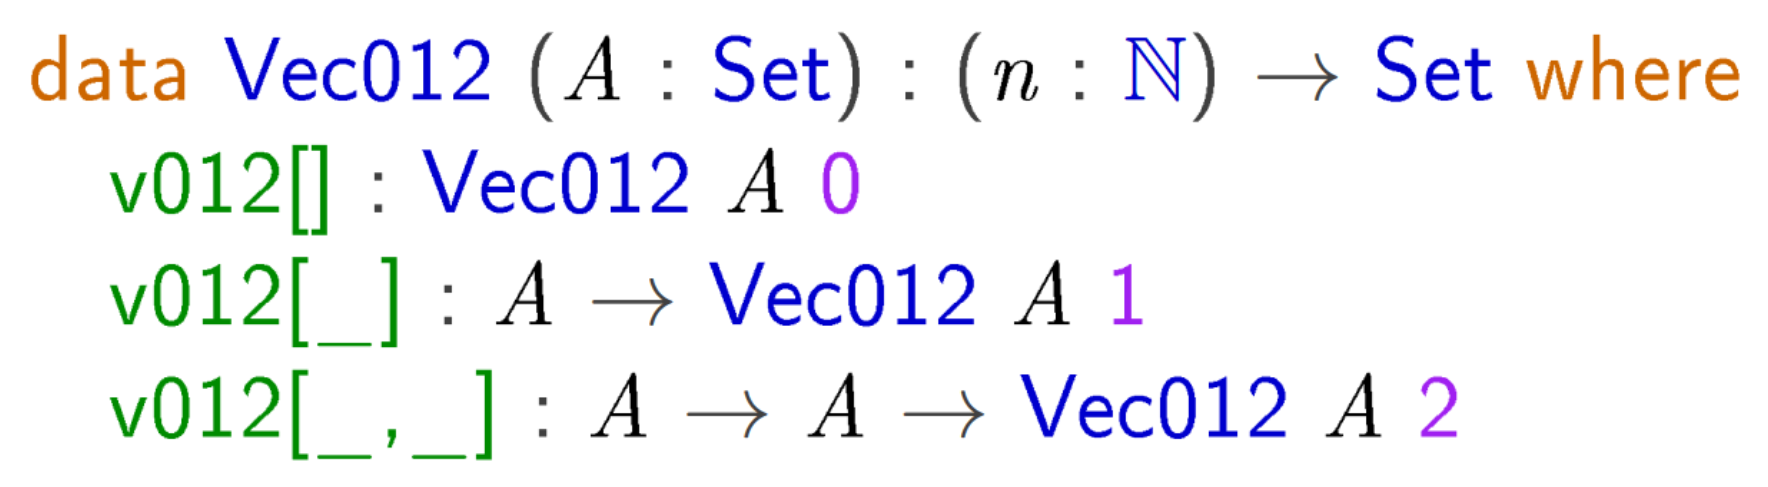
\includegraphics[scale=0.4]{img/vec012}
\end{figure}
\end{frame}



\begin{frame}{Tipos dependientes}
\begin{figure}
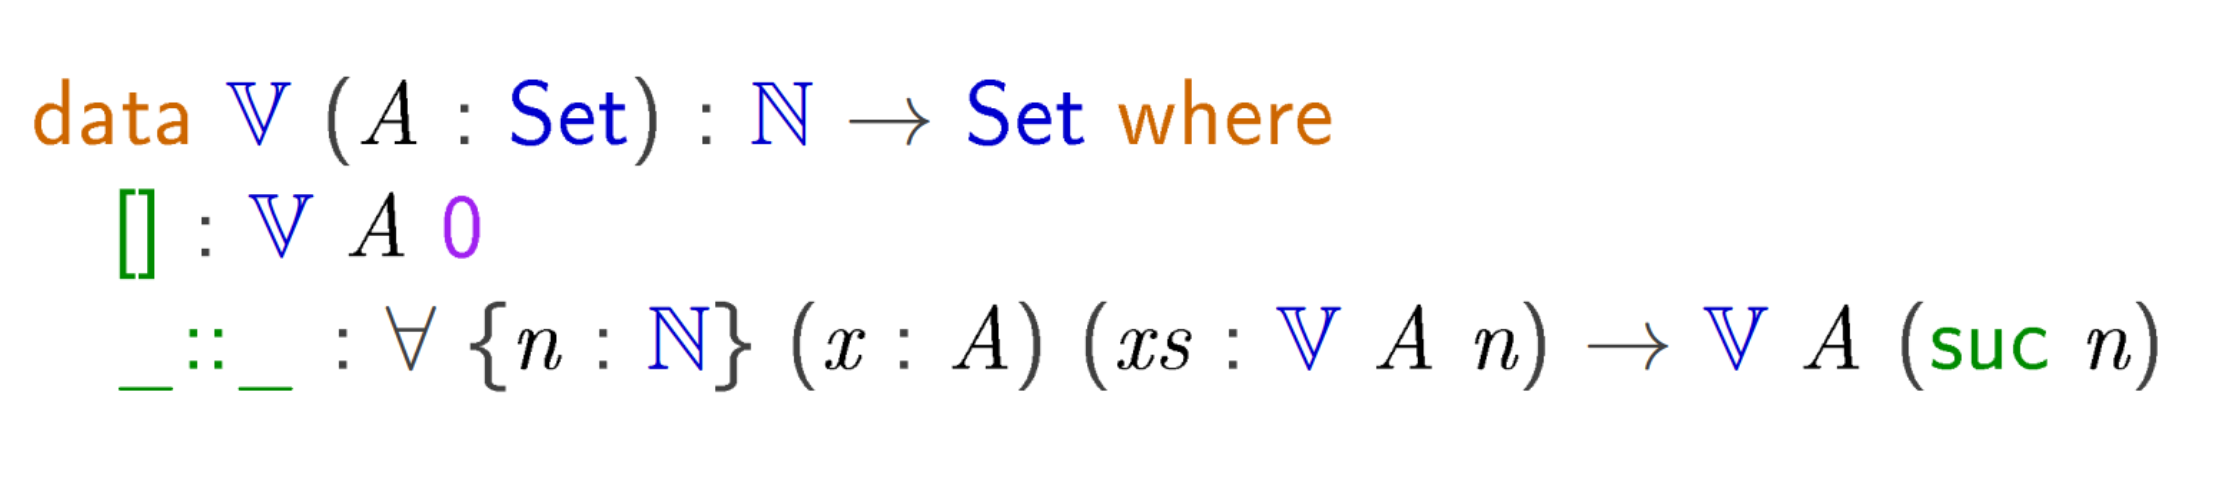
\includegraphics[scale=0.4]{img/vec}
\end{figure}
\end{frame}



\begin{frame}{La igualdad}
\begin{figure}
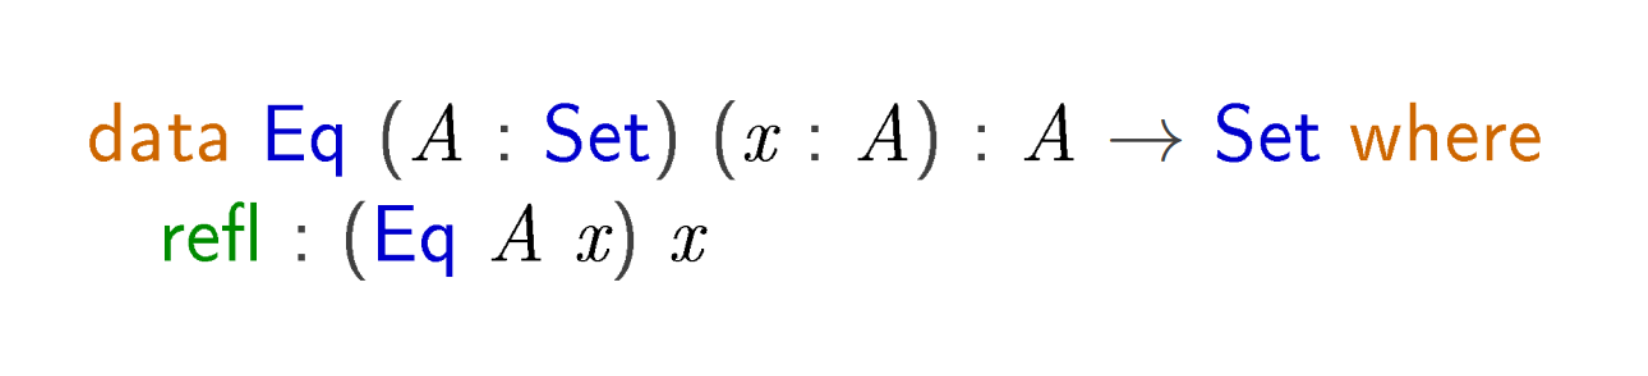
\includegraphics[scale=0.5]{img/eq}
\end{figure}
\end{frame}

\begin{frame}{La igualdad}
\begin{figure}
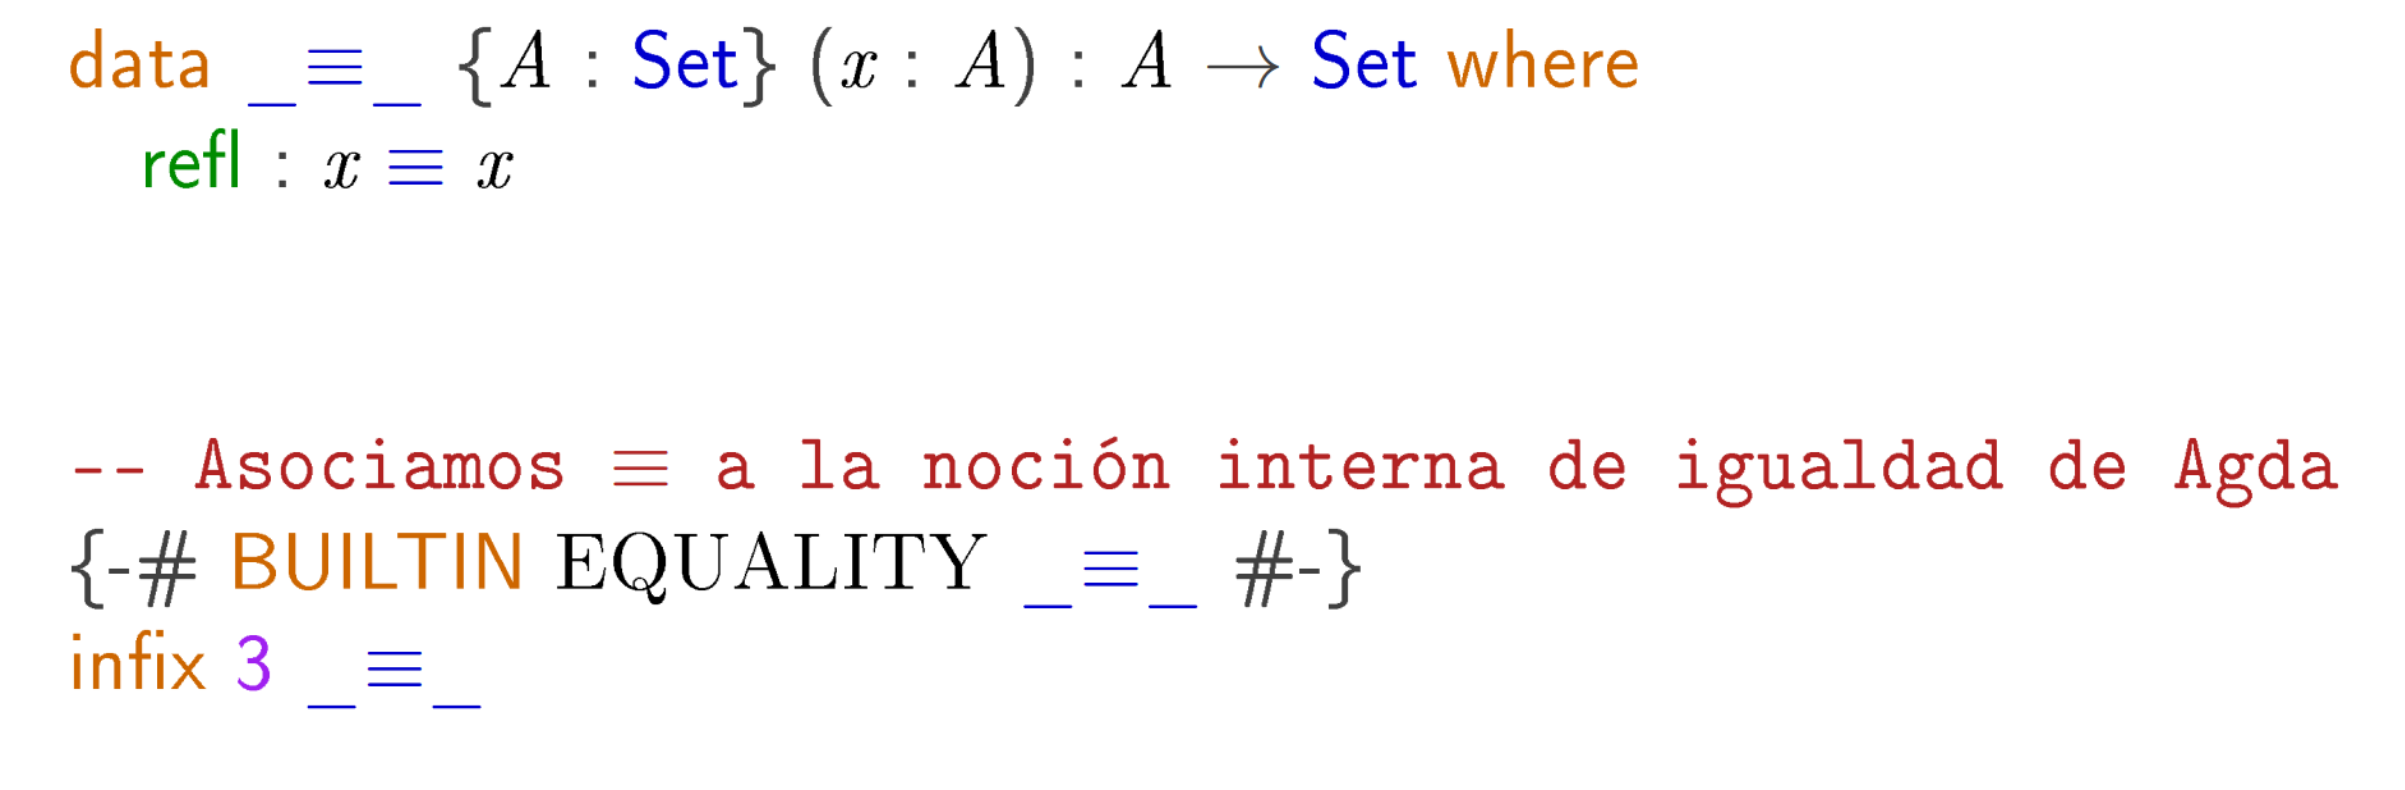
\includegraphics[scale=0.4]{img/equality}
\end{figure}
\end{frame}


\begin{frame}{Igualdad proposicional y definicional}
\begin{figure}
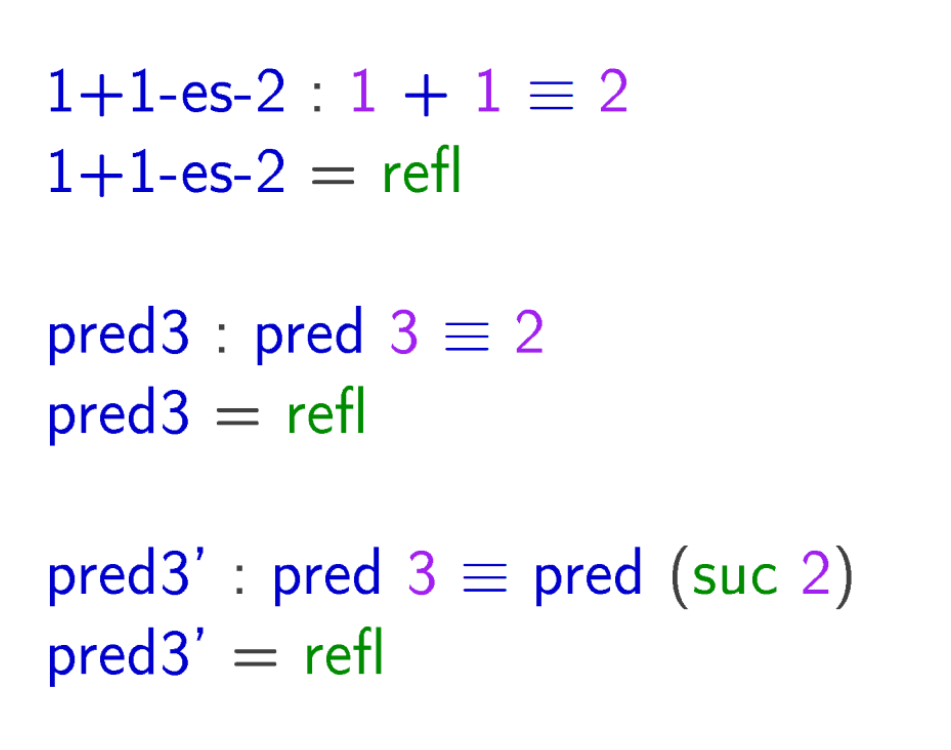
\includegraphics[scale=0.7]{img/propeq}
\end{figure}
\end{frame}



\begin{frame}{Algunas propiedades de la igualdad}
\begin{figure}
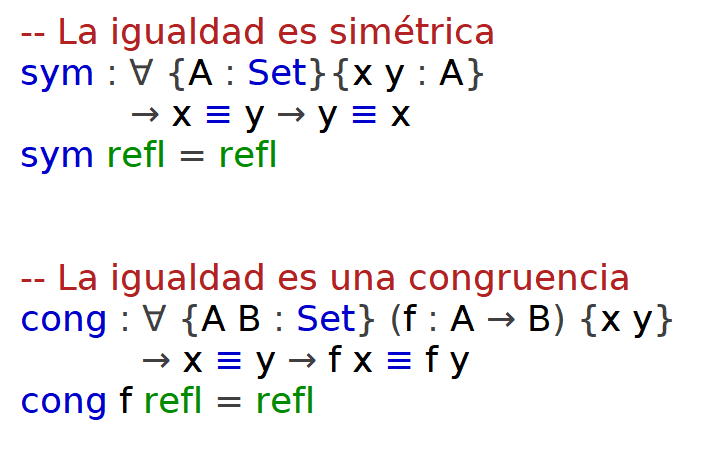
\includegraphics[scale=0.9]{img/congsym}
\end{figure}
\end{frame}


\begin{frame}{Demostraciones}
\begin{figure}
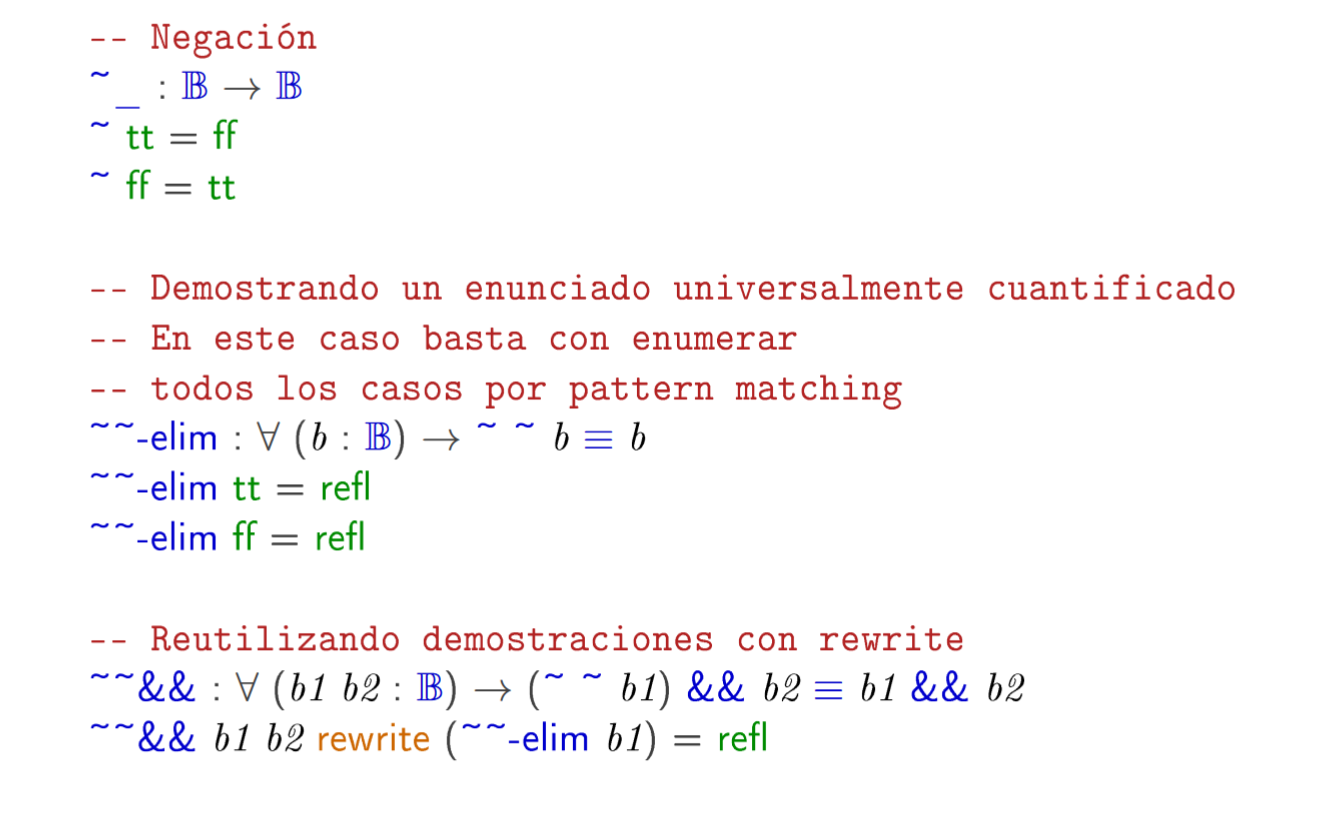
\includegraphics[scale=0.7]{img/dems}
\end{figure}
\end{frame}



\begin{frame}{Demostraciones}
\begin{figure}
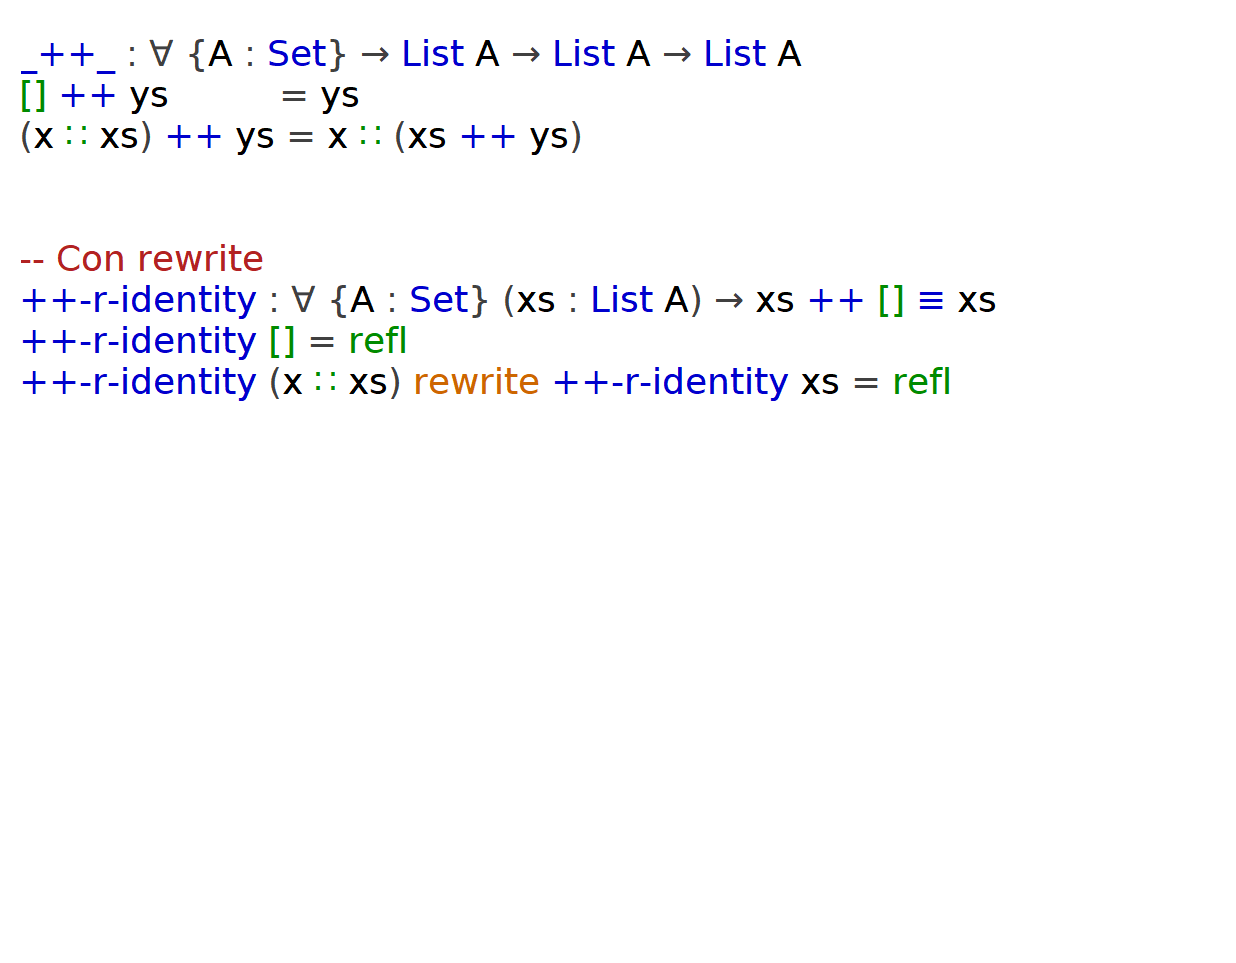
\includegraphics[scale=0.7]{img/reasoning01}
\end{figure}
\end{frame}



\begin{frame}{Demostraciones}
\begin{figure}
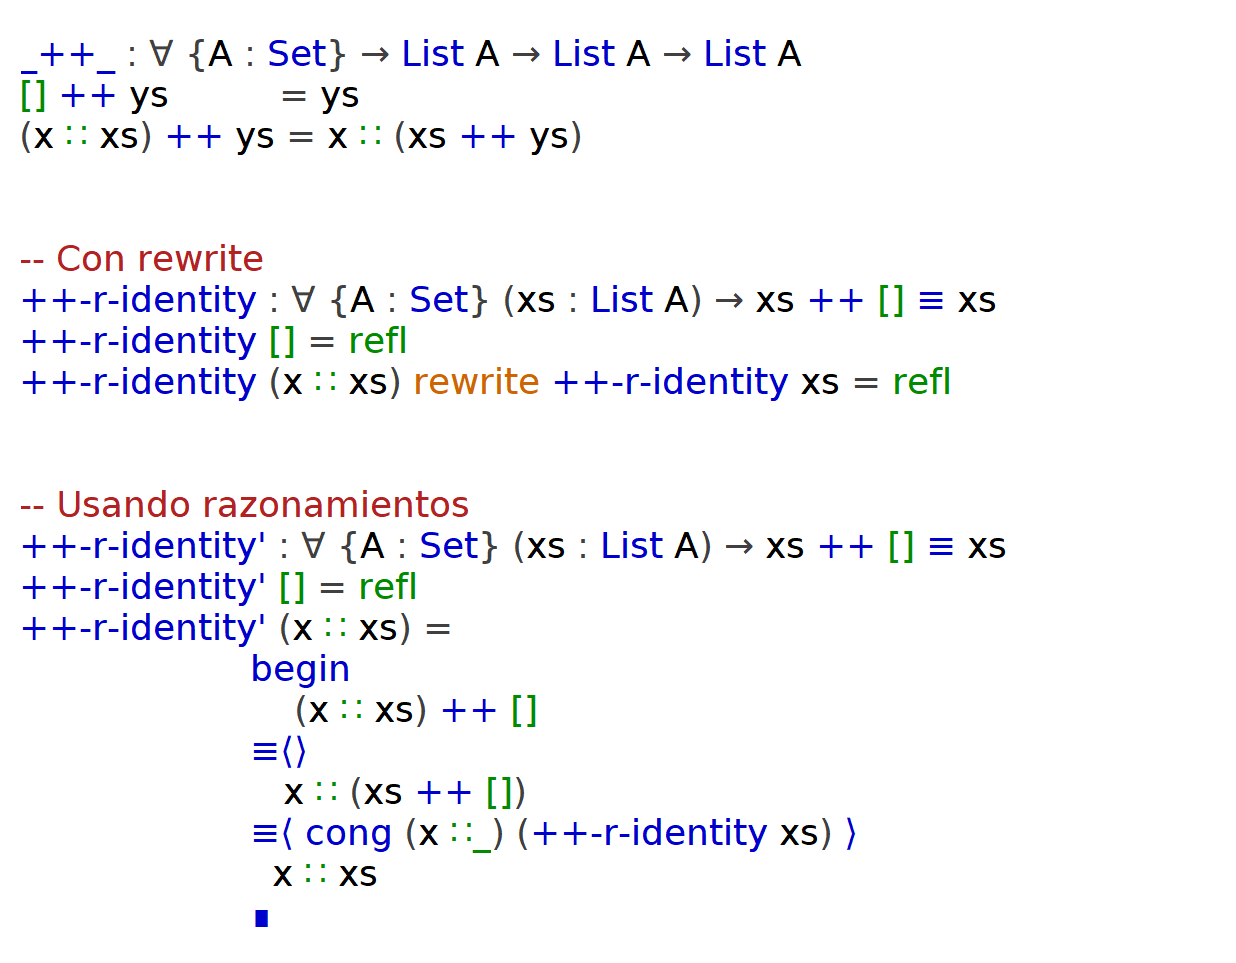
\includegraphics[scale=0.7]{img/reasoning02}
\end{figure}
\end{frame}

\begin{frame}{Razonamientos con igualdad}
\begin{figure}
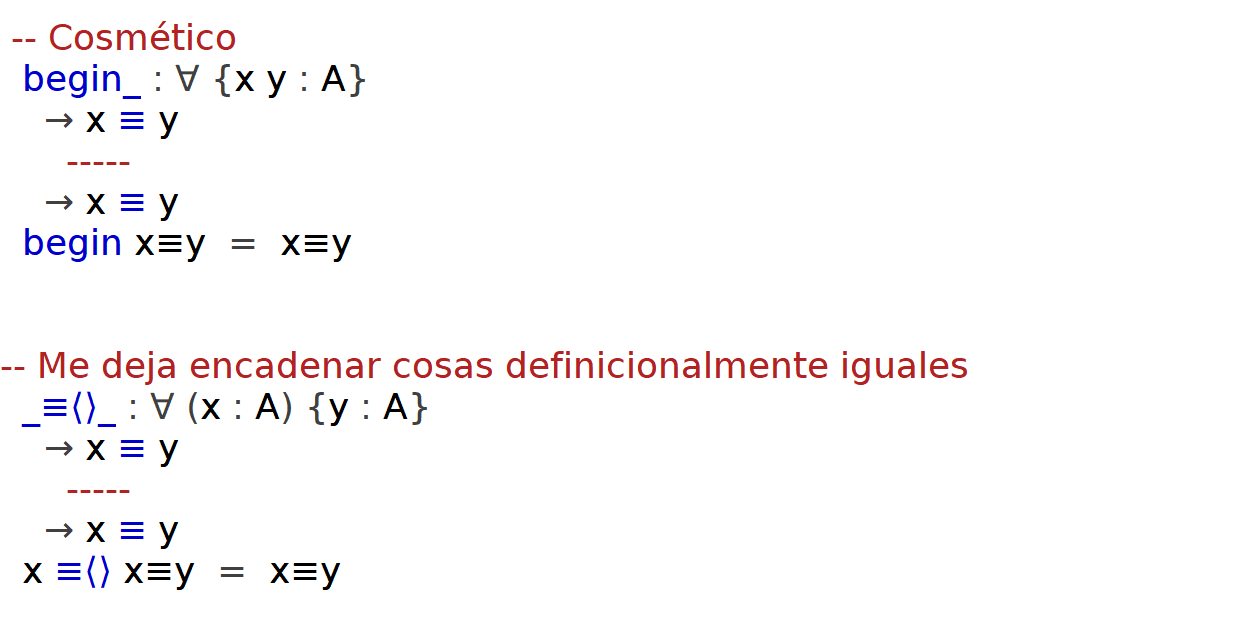
\includegraphics[scale=0.7]{img/eq-reasoning}
\end{figure}
\end{frame}

\begin{frame}{Razonamientos con igualdad}
\begin{figure}
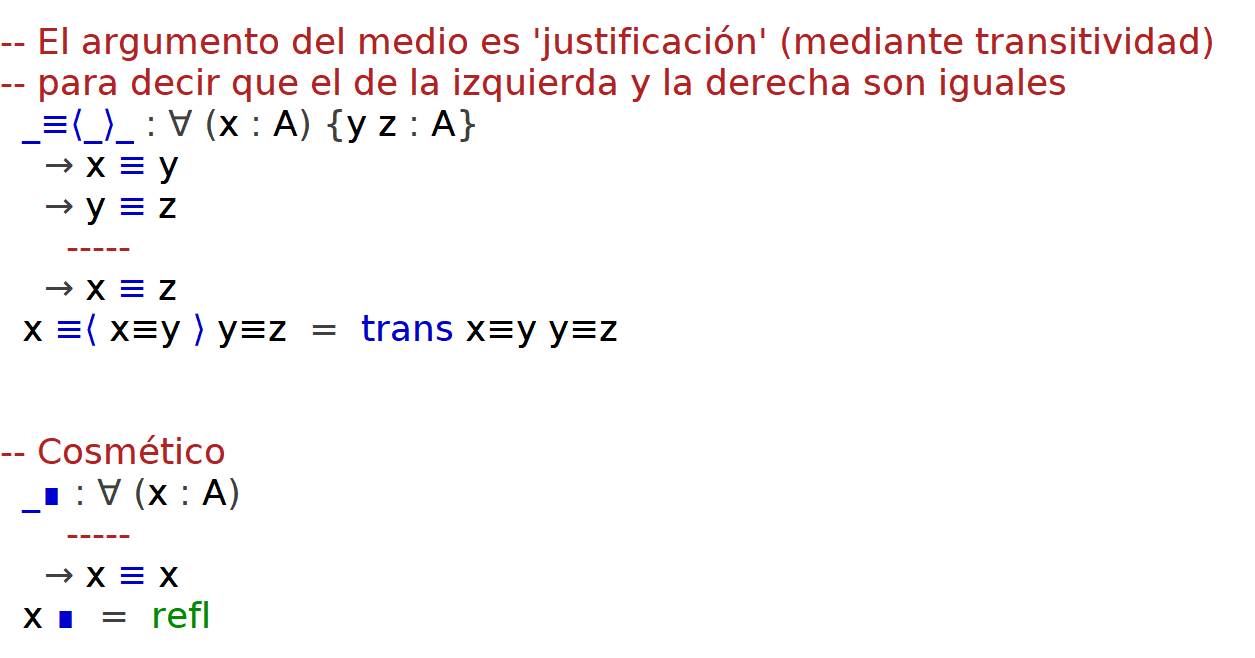
\includegraphics[scale=0.7]{img/eq-reasoning02}
\end{figure}
\end{frame}


\begin{frame}{Más demostraciones}
\begin{figure}
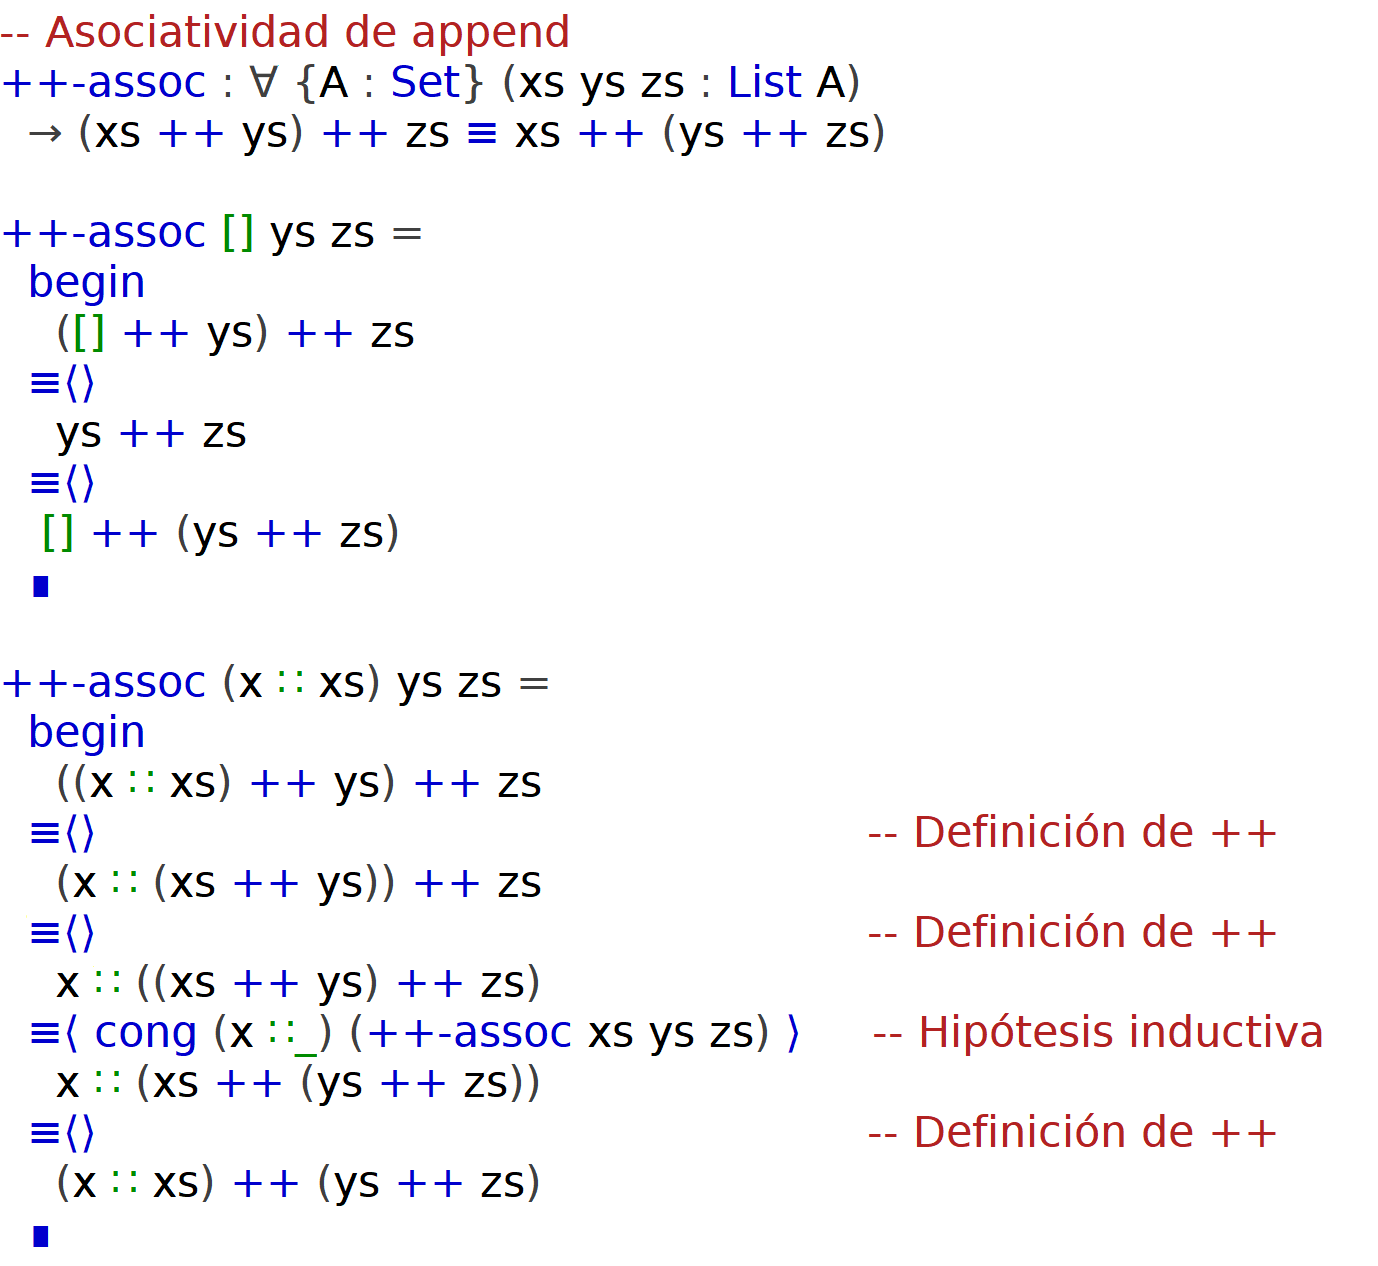
\includegraphics[scale=0.5]{img/assoc}
\end{figure}
\end{frame}

\begin{frame}{Más demostraciones}
\begin{figure}
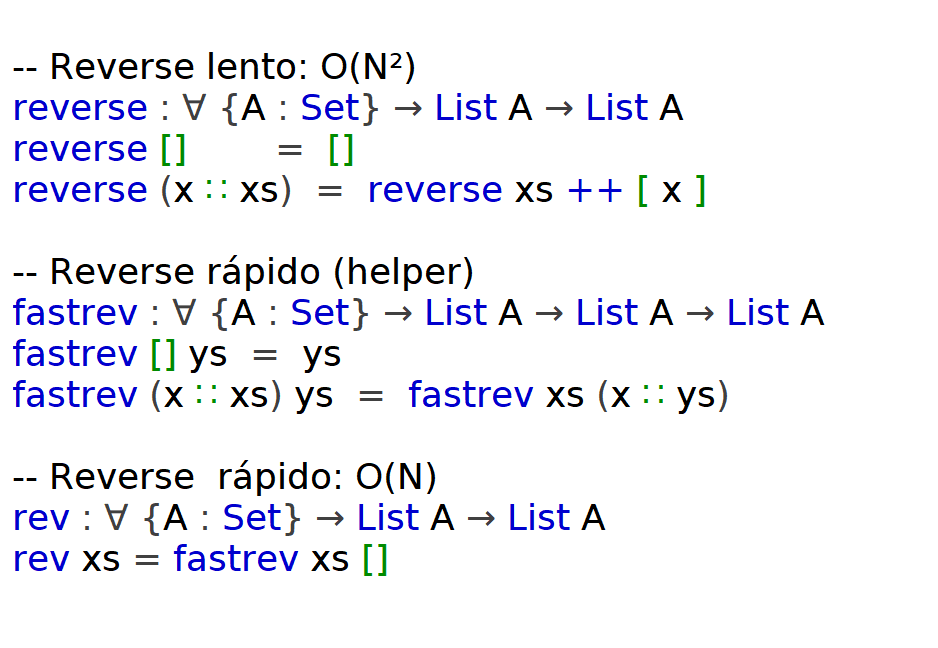
\includegraphics[scale=0.65]{img/rev-def}
\end{figure}

Quiero demostrar que \texttt{reverse} y \texttt{rev} hacen lo mismo...
\end{frame}



\begin{frame}{Más demostraciones}
\begin{figure}
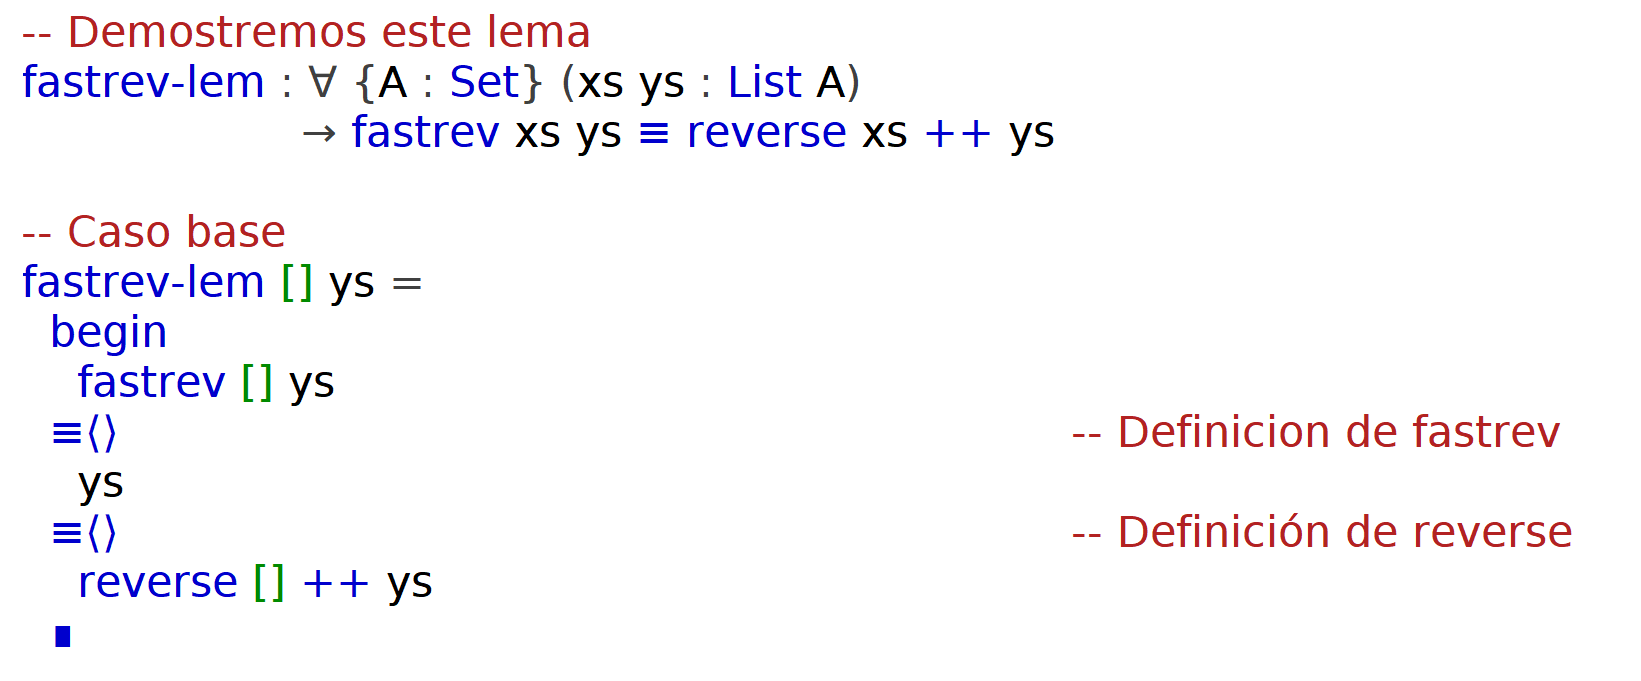
\includegraphics[scale=0.55]{img/fastrev-lem01}
\end{figure}
\end{frame}


\begin{frame}{Más demostraciones}
\begin{figure}
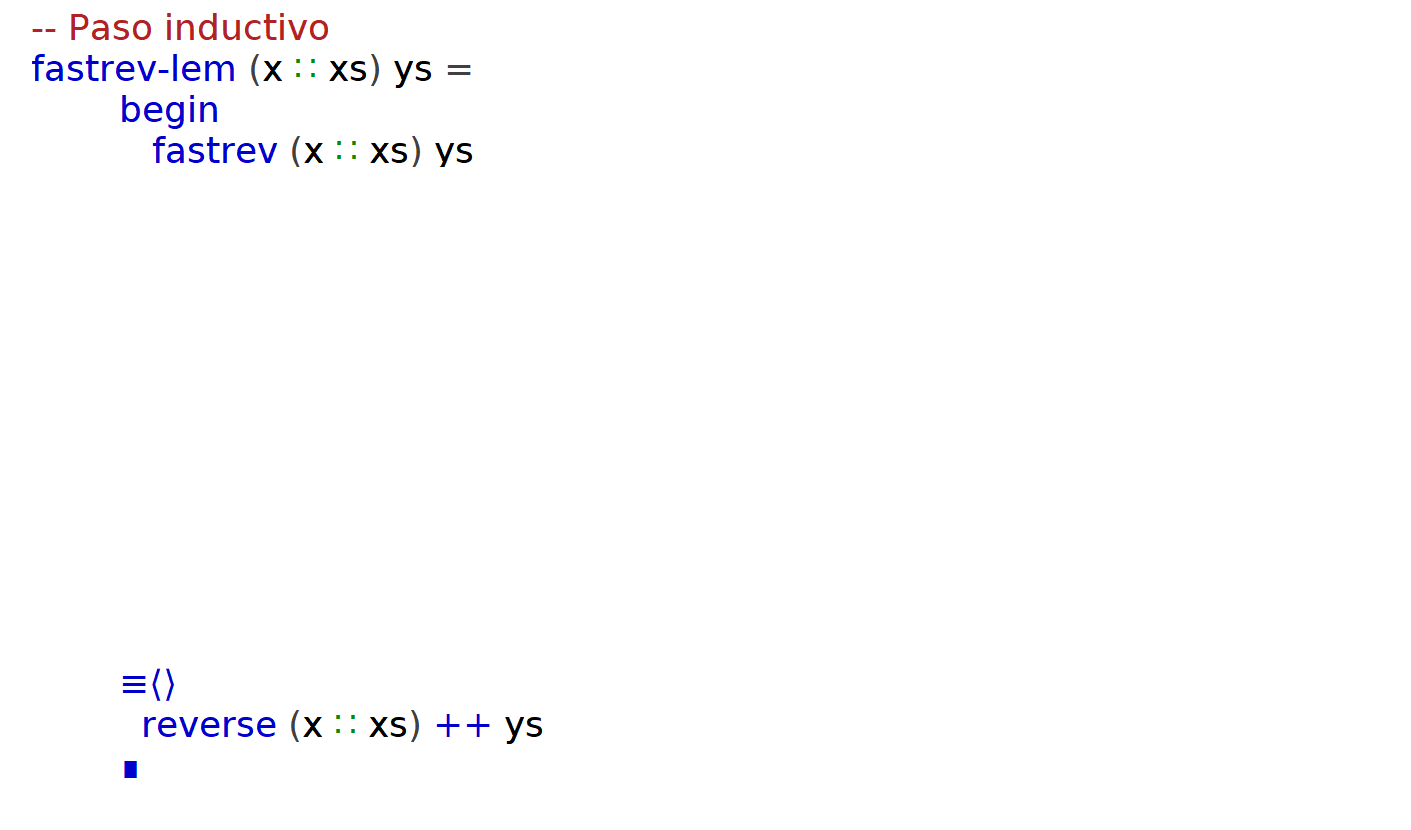
\includegraphics[scale=0.65]{img/fastrev-lem-dem01}
\end{figure}
\end{frame}

\begin{frame}{Más demostraciones}
\begin{figure}
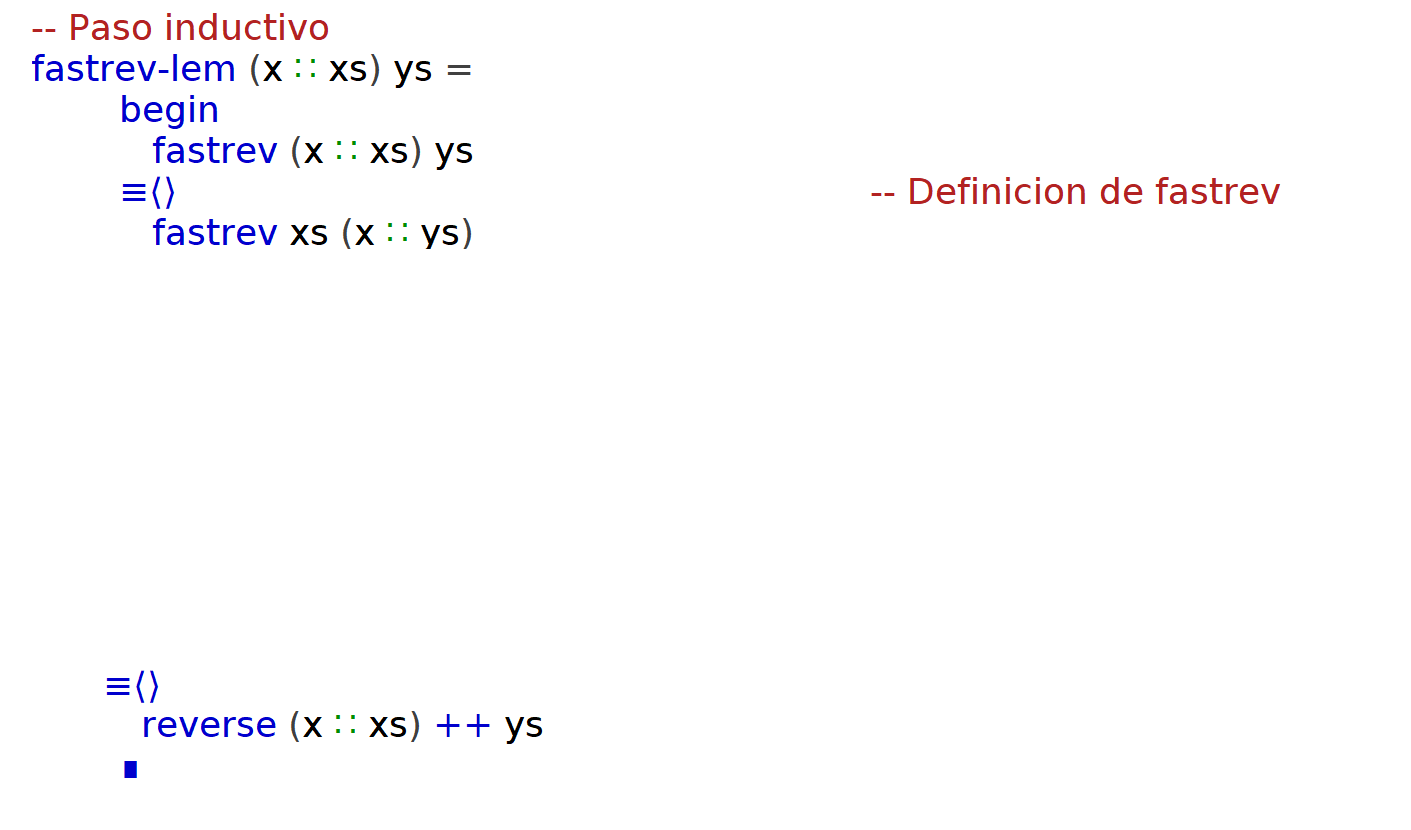
\includegraphics[scale=0.65]{img/fastrev-lem-dem02}
\end{figure}
\end{frame}


\begin{frame}{Más demostraciones}
\begin{figure}
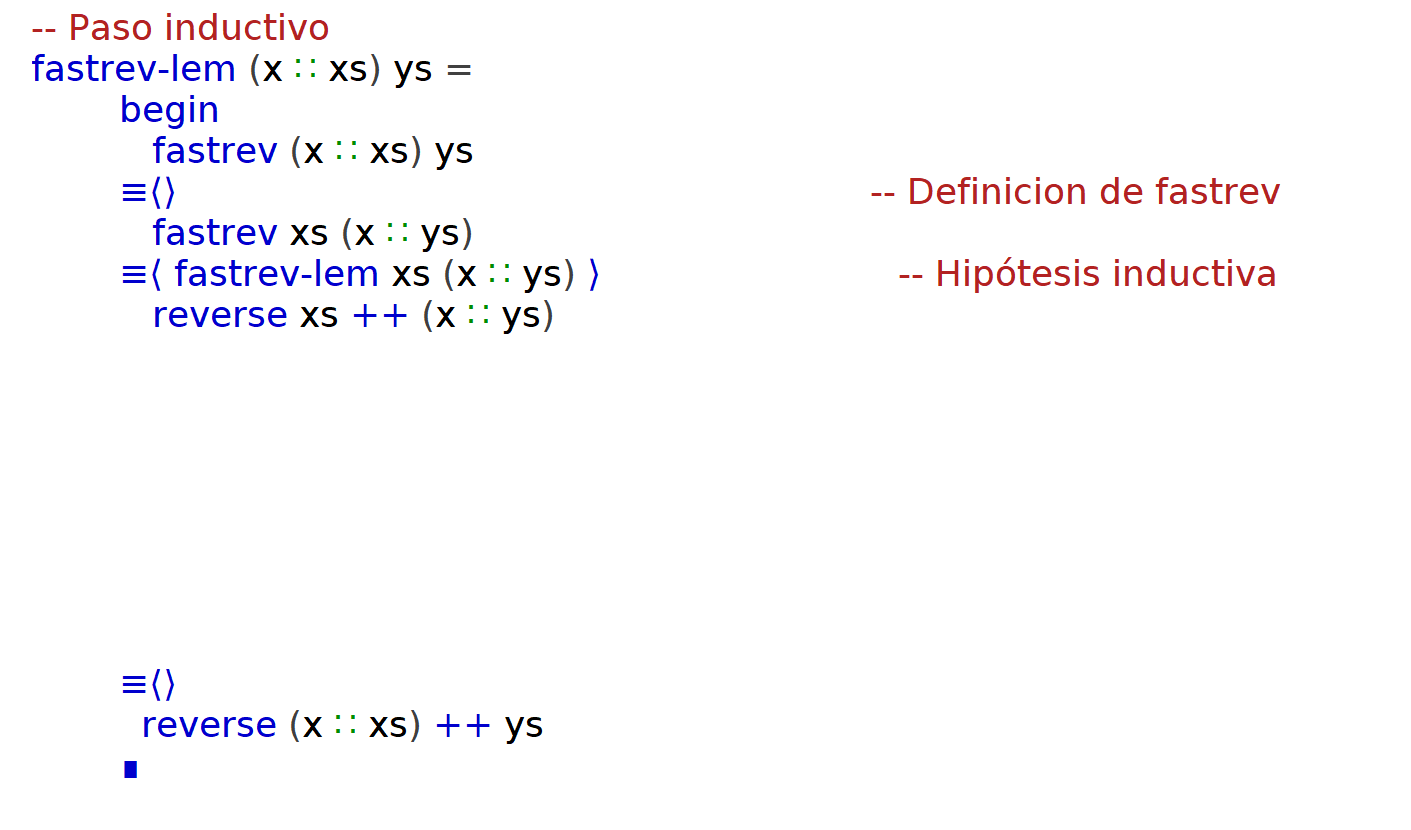
\includegraphics[scale=0.65]{img/fastrev-lem-dem03}
\end{figure}
\end{frame}


\begin{frame}{Más demostraciones}
\begin{figure}
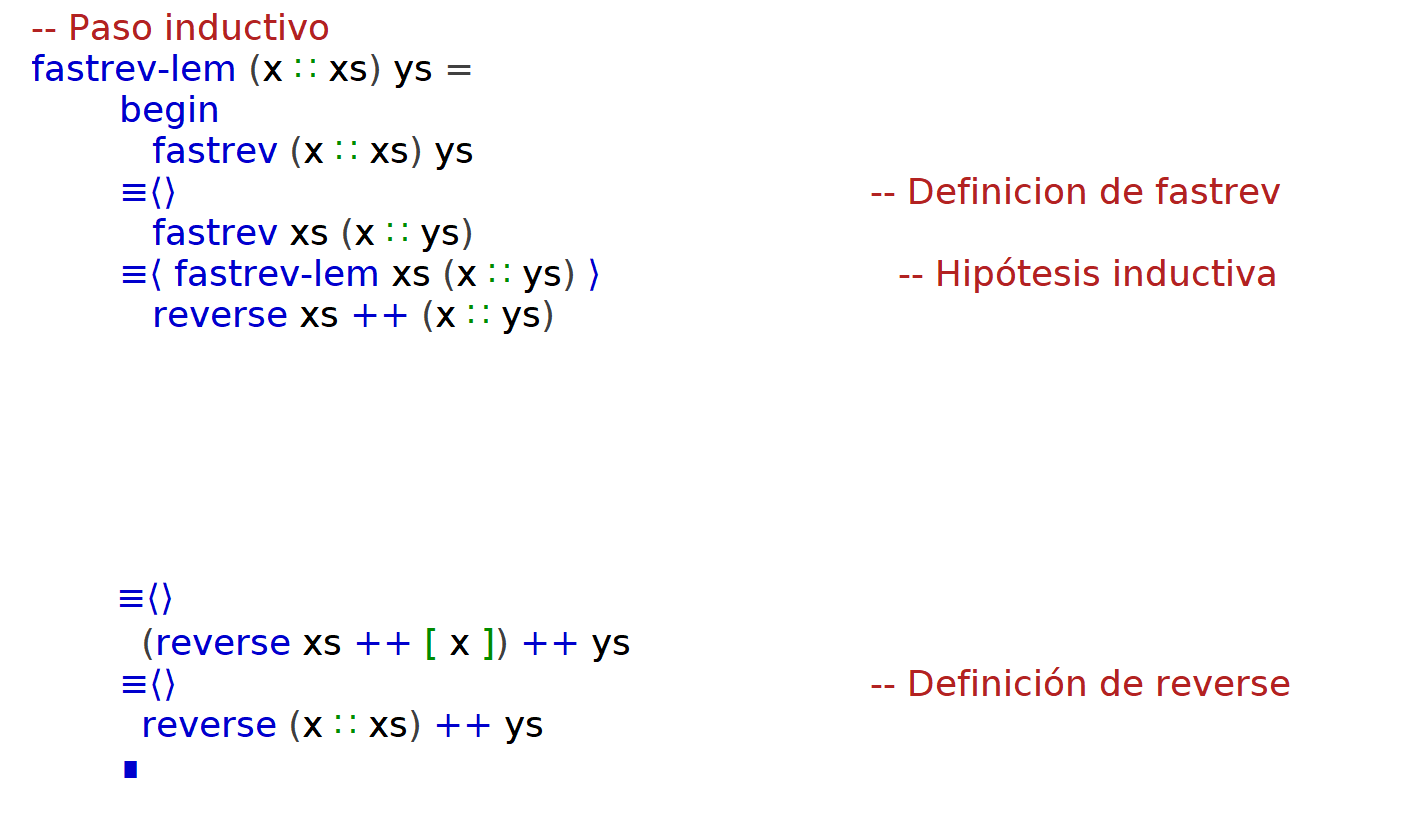
\includegraphics[scale=0.65]{img/fastrev-lem-dem04}
\end{figure}
\end{frame}


\begin{frame}{Más demostraciones}
\begin{figure}
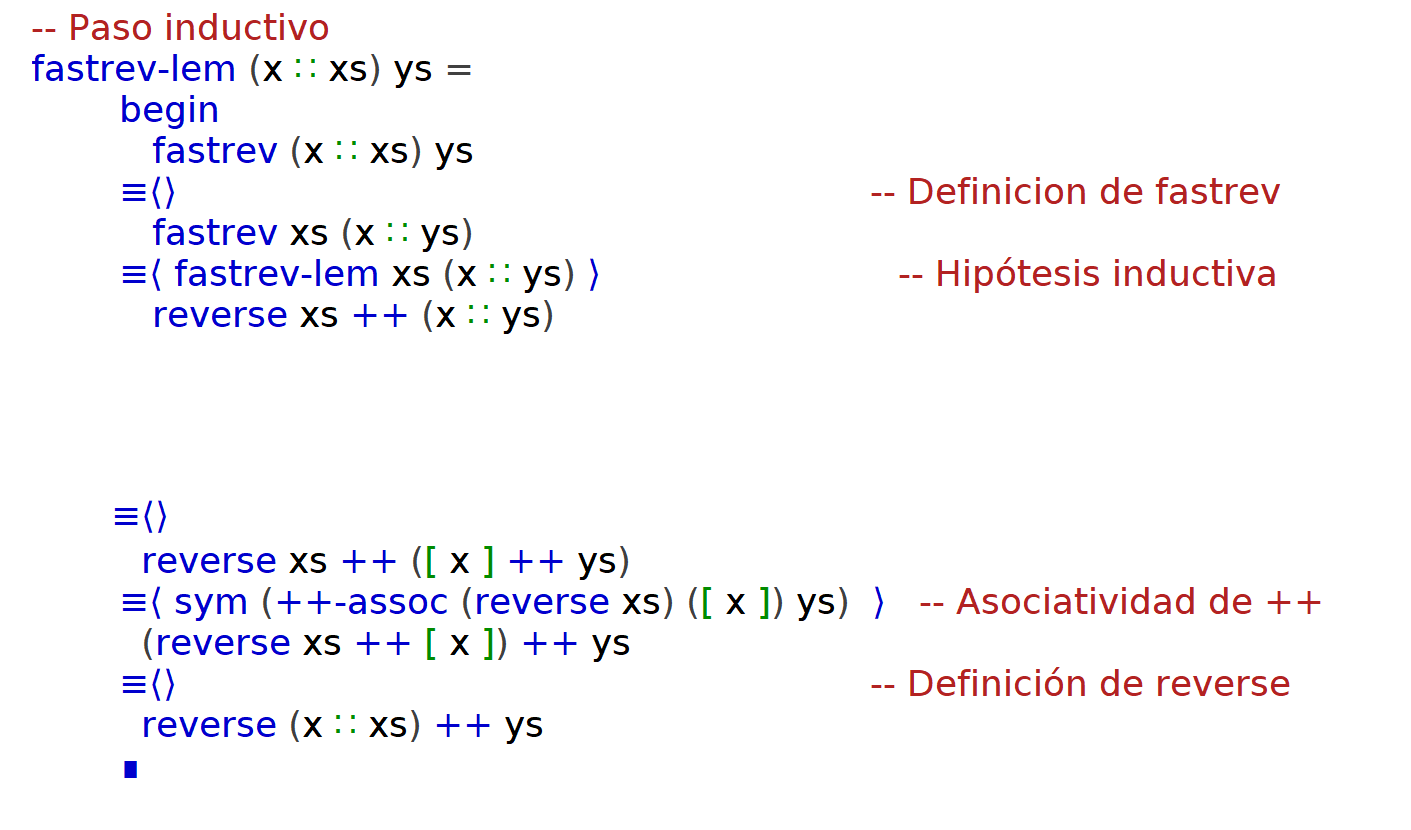
\includegraphics[scale=0.65]{img/fastrev-lem-dem05}
\end{figure}
\end{frame}


\begin{frame}{Más demostraciones}
\begin{figure}
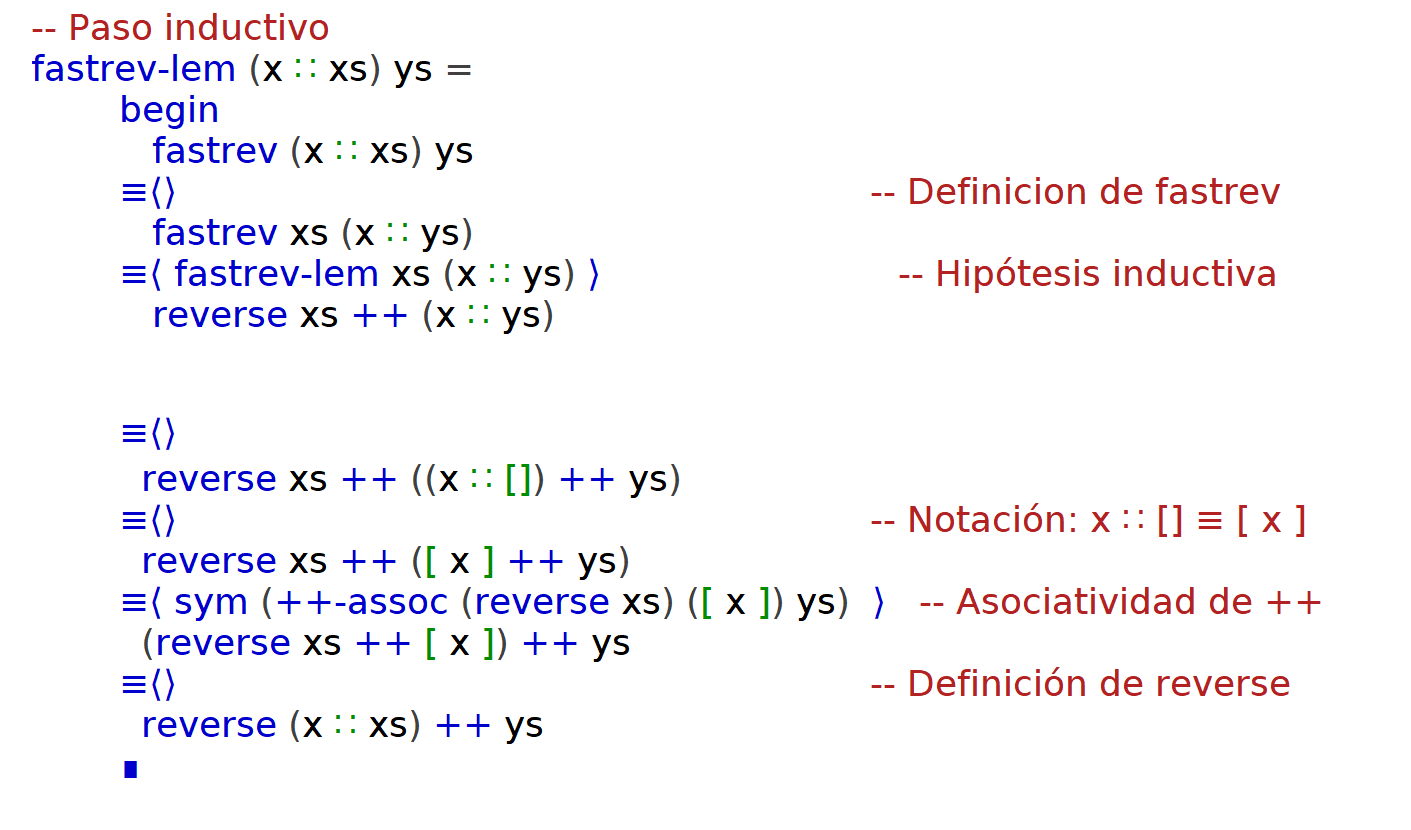
\includegraphics[scale=0.65]{img/fastrev-lem-dem05b}
\end{figure}
\end{frame}


\begin{frame}{Más demostraciones}
\begin{figure}
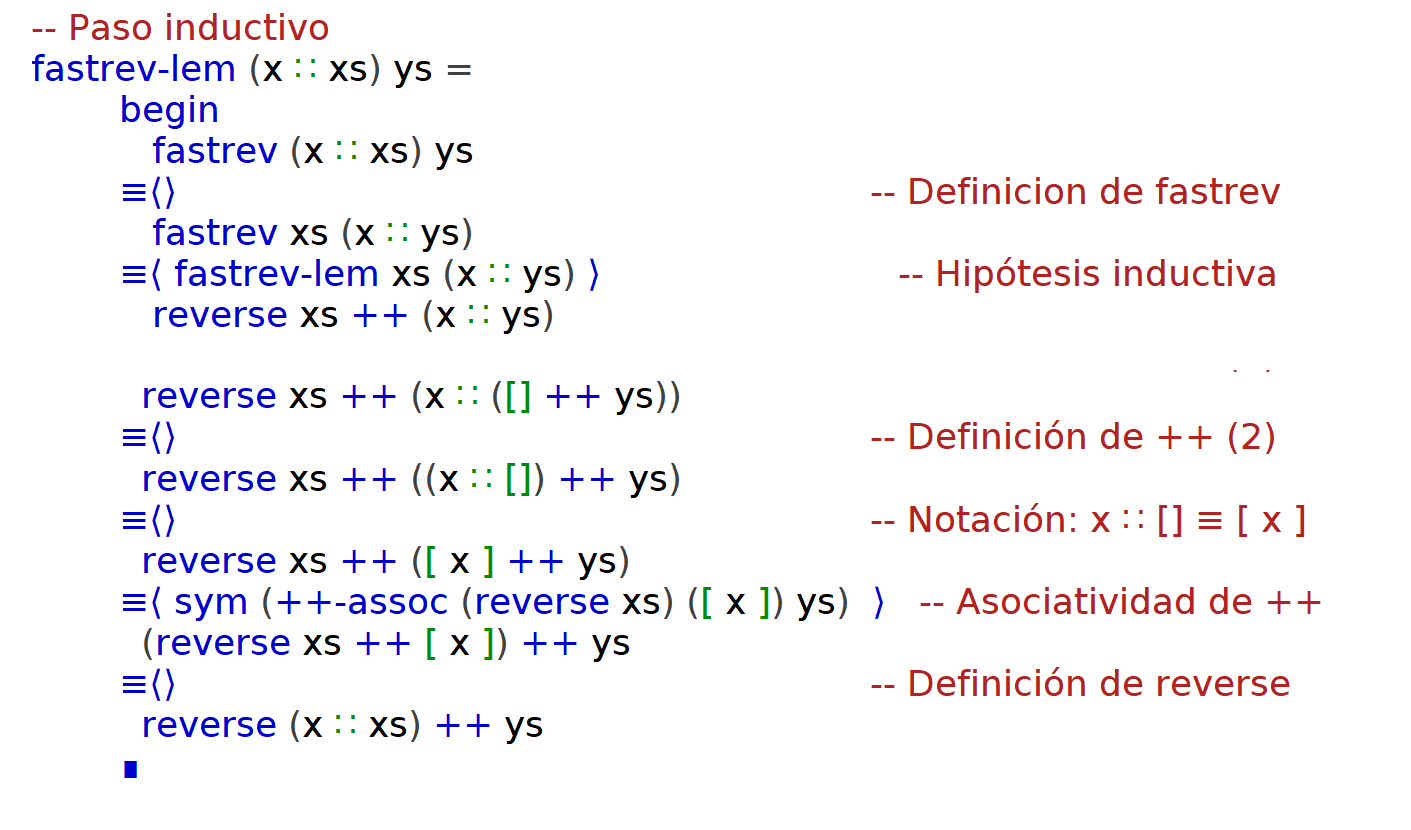
\includegraphics[scale=0.65]{img/fastrev-lem-dem05c}
\end{figure}
\end{frame}


\begin{frame}{Más demostraciones}
\begin{figure}
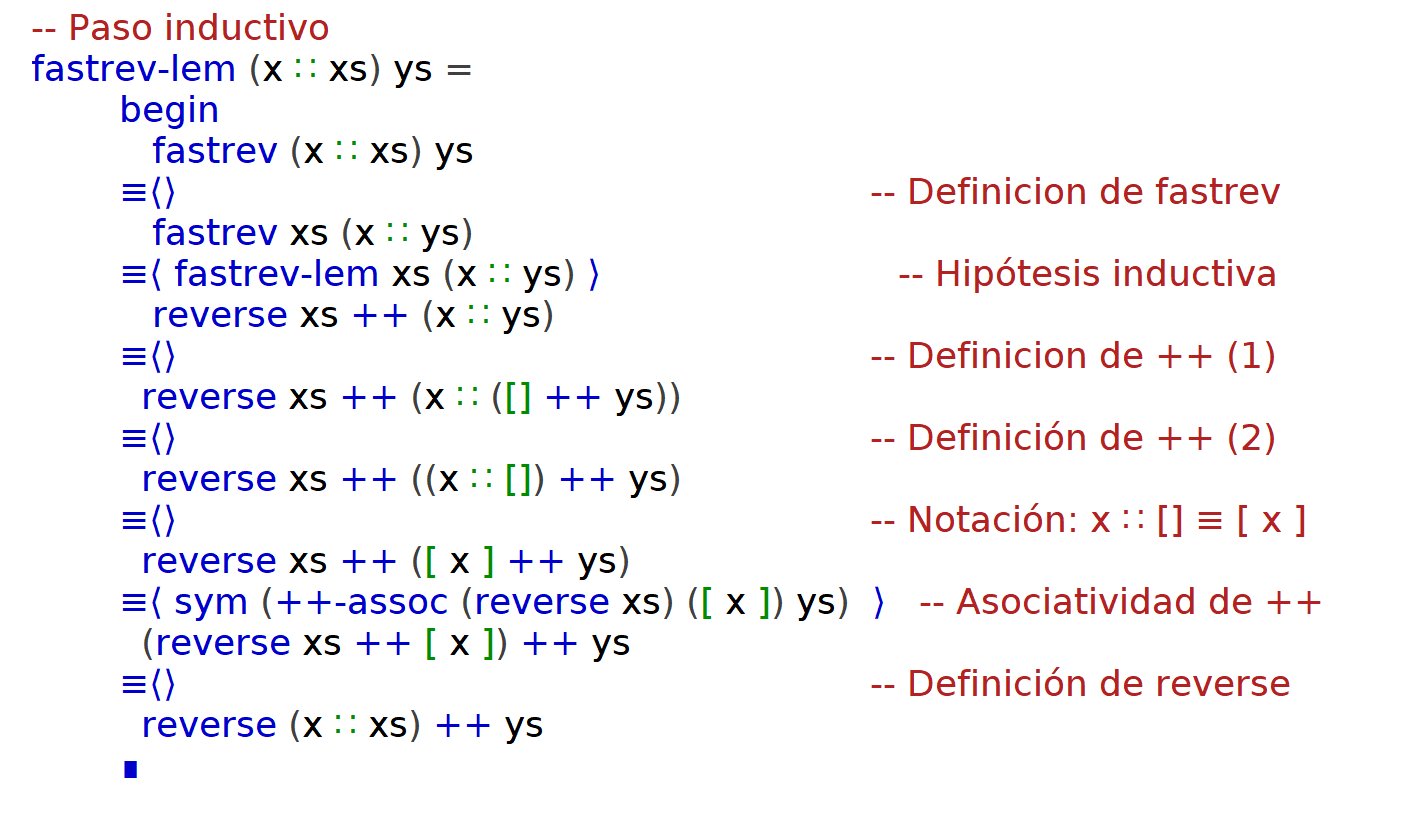
\includegraphics[scale=0.65]{img/fastrev-lem-dem06}
\end{figure}
\end{frame}


\begin{frame}{Más demostraciones}
\begin{figure}
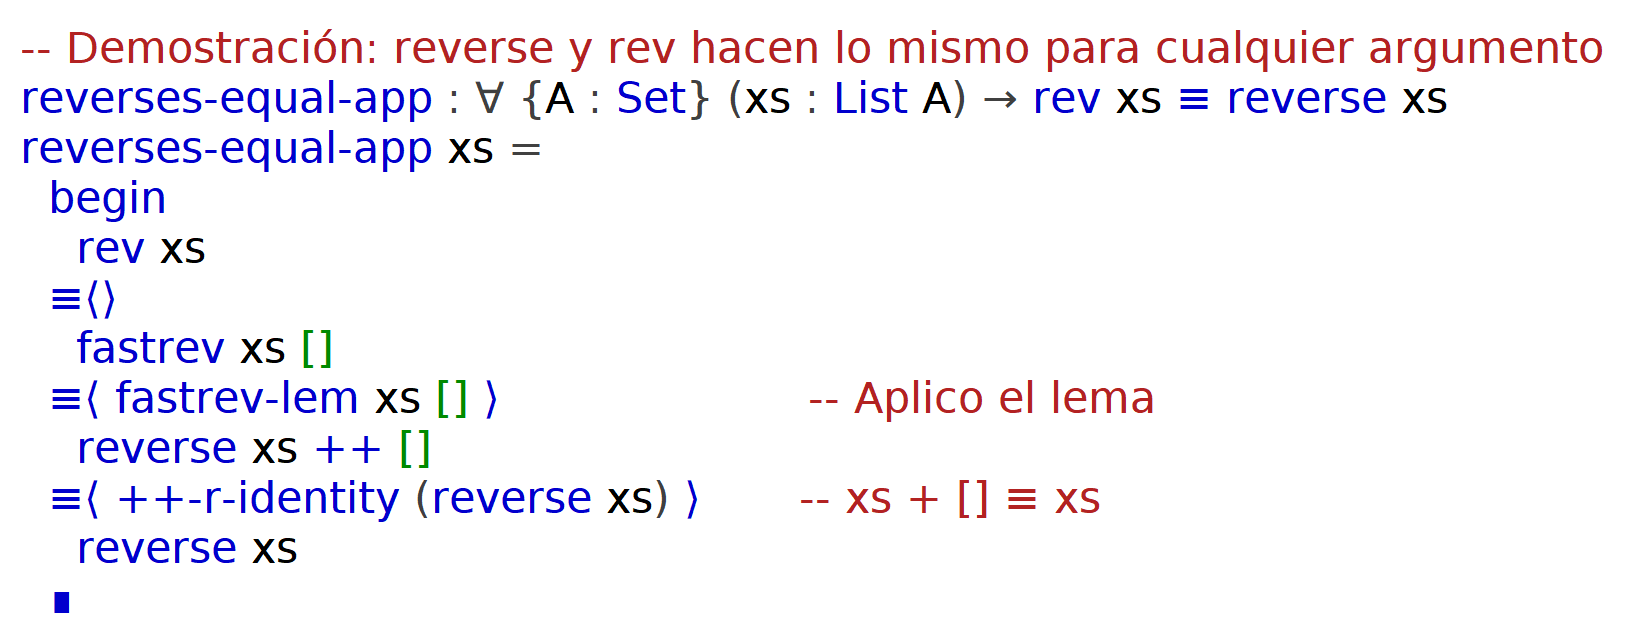
\includegraphics[scale=0.55]{img/rev-thm}
\end{figure}
\end{frame}


\begin{frame}{Extensionalidad como postulado}
\begin{figure}
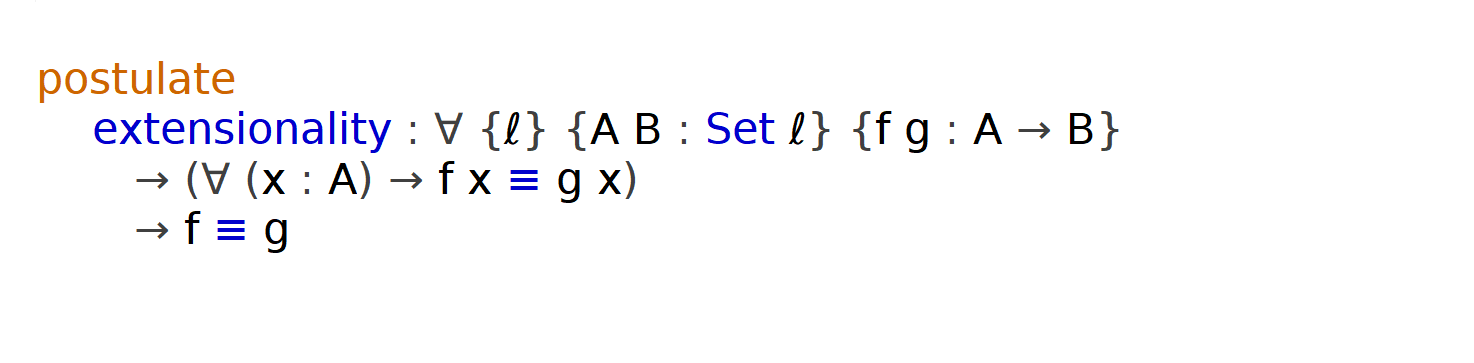
\includegraphics[scale=0.6]{img/extensionality}
\end{figure}
\bit
\item No se puede demostrar extensionalidad dentro de Agda
\item Sin embargo el postulado es consistente con Agda así que podemos usarlo sin problemas
\eit
\end{frame}


\begin{frame}{Extensionalidad como postulado}
\begin{figure}
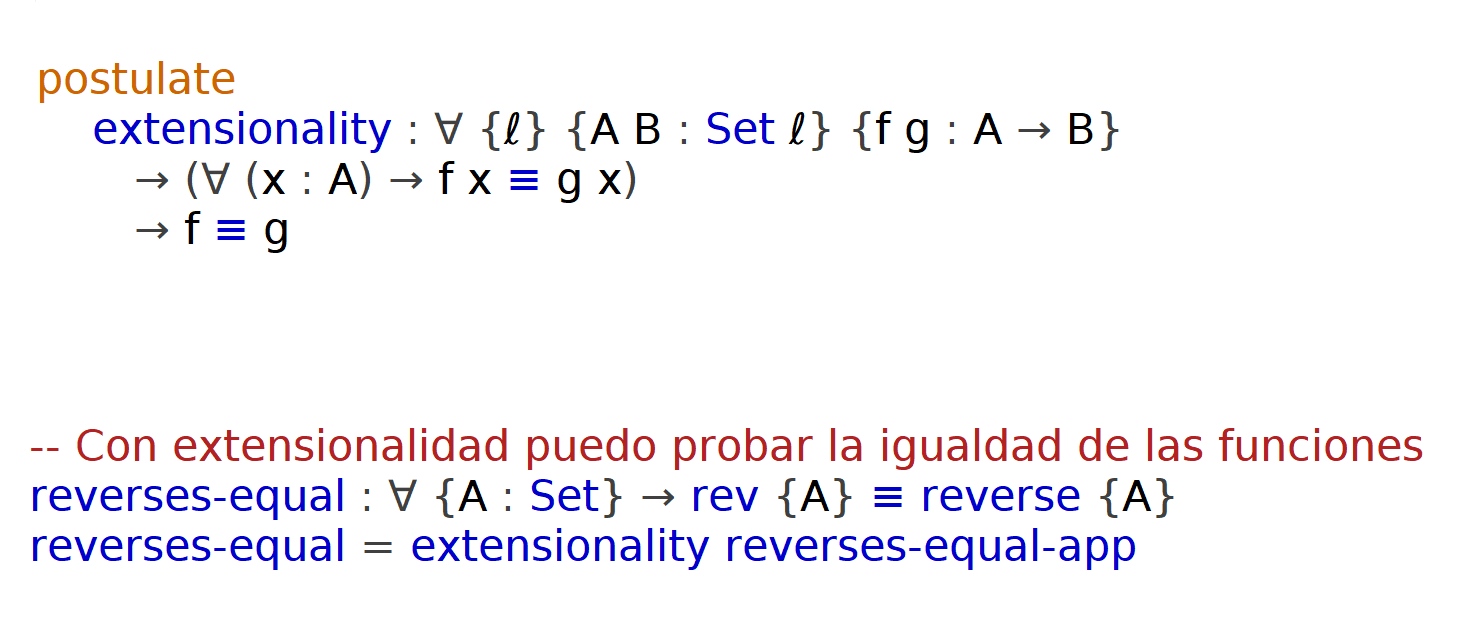
\includegraphics[scale=0.6]{img/extensionality02}
\end{figure}
\end{frame}

\begin{frame}{Verificación interna}

\bit
\item Hasta ahora definimos tipos de datos (como \texttt{List}) y programas (como $++$ ) y luego demostramos propiedades sobre los mismos. 

\biti
\item Esto podría llamarse \textit{verificación externa}: las demostraciones son externas a los programas.
\eit


\item En contraste, podemos considerar un estilo de verificación que podemos llamar \textit{verificación interna} en donde expresamos las proposiciones \textit{dentro de los mismos tipos de datos y programas}

\item La idea es escribir tipos y funciones más expresivos: la corrección de las funciones y las invariantes de las estructuras de datos están garantizadas por el propio tipo.

\eit
\end{frame}

\begin{frame}{Vectores: el tipo $\mathbb{V}$}
\begin{figure}
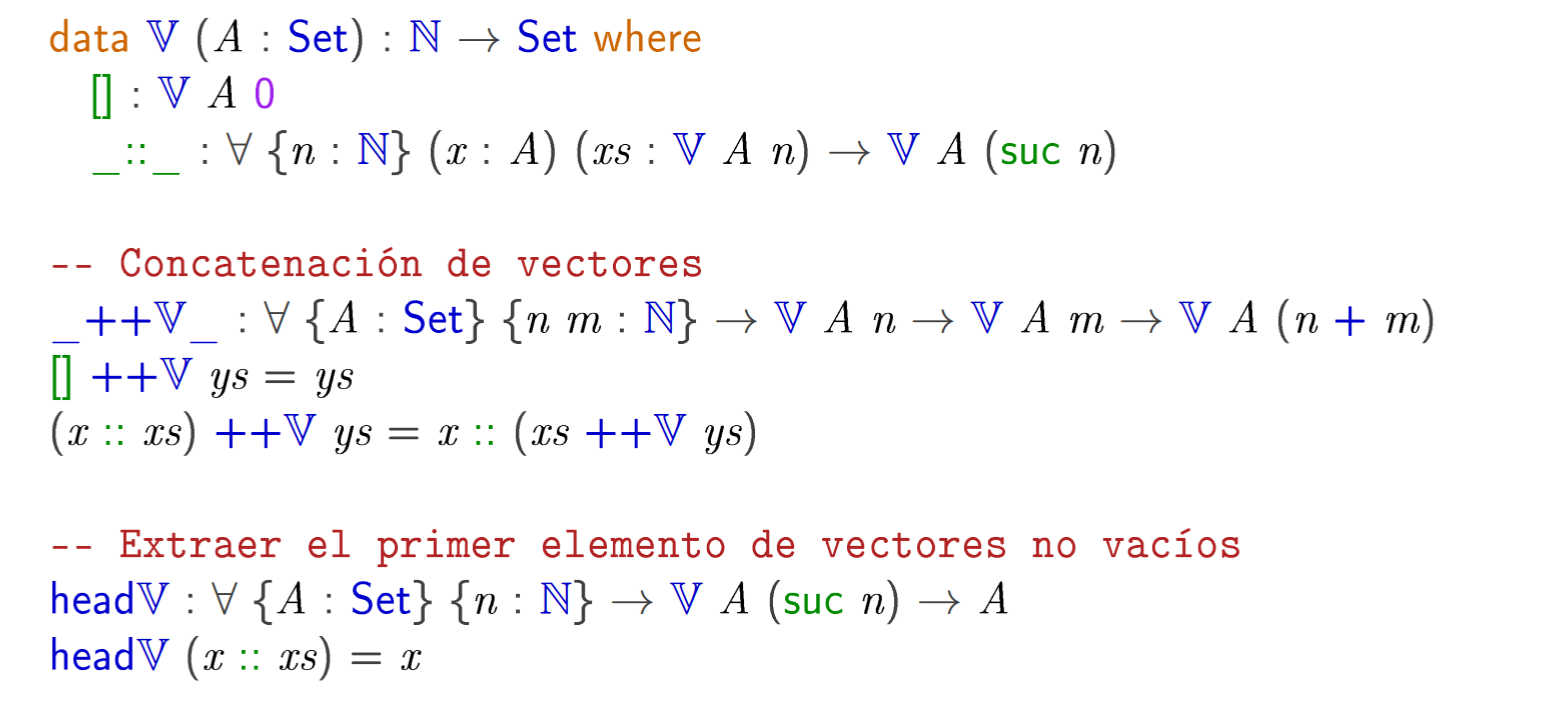
\includegraphics[scale=0.6]{img/vector-vi}
\end{figure}

\end{frame}


\begin{frame}{Árboles binarios de búsqueda}
\begin{figure}
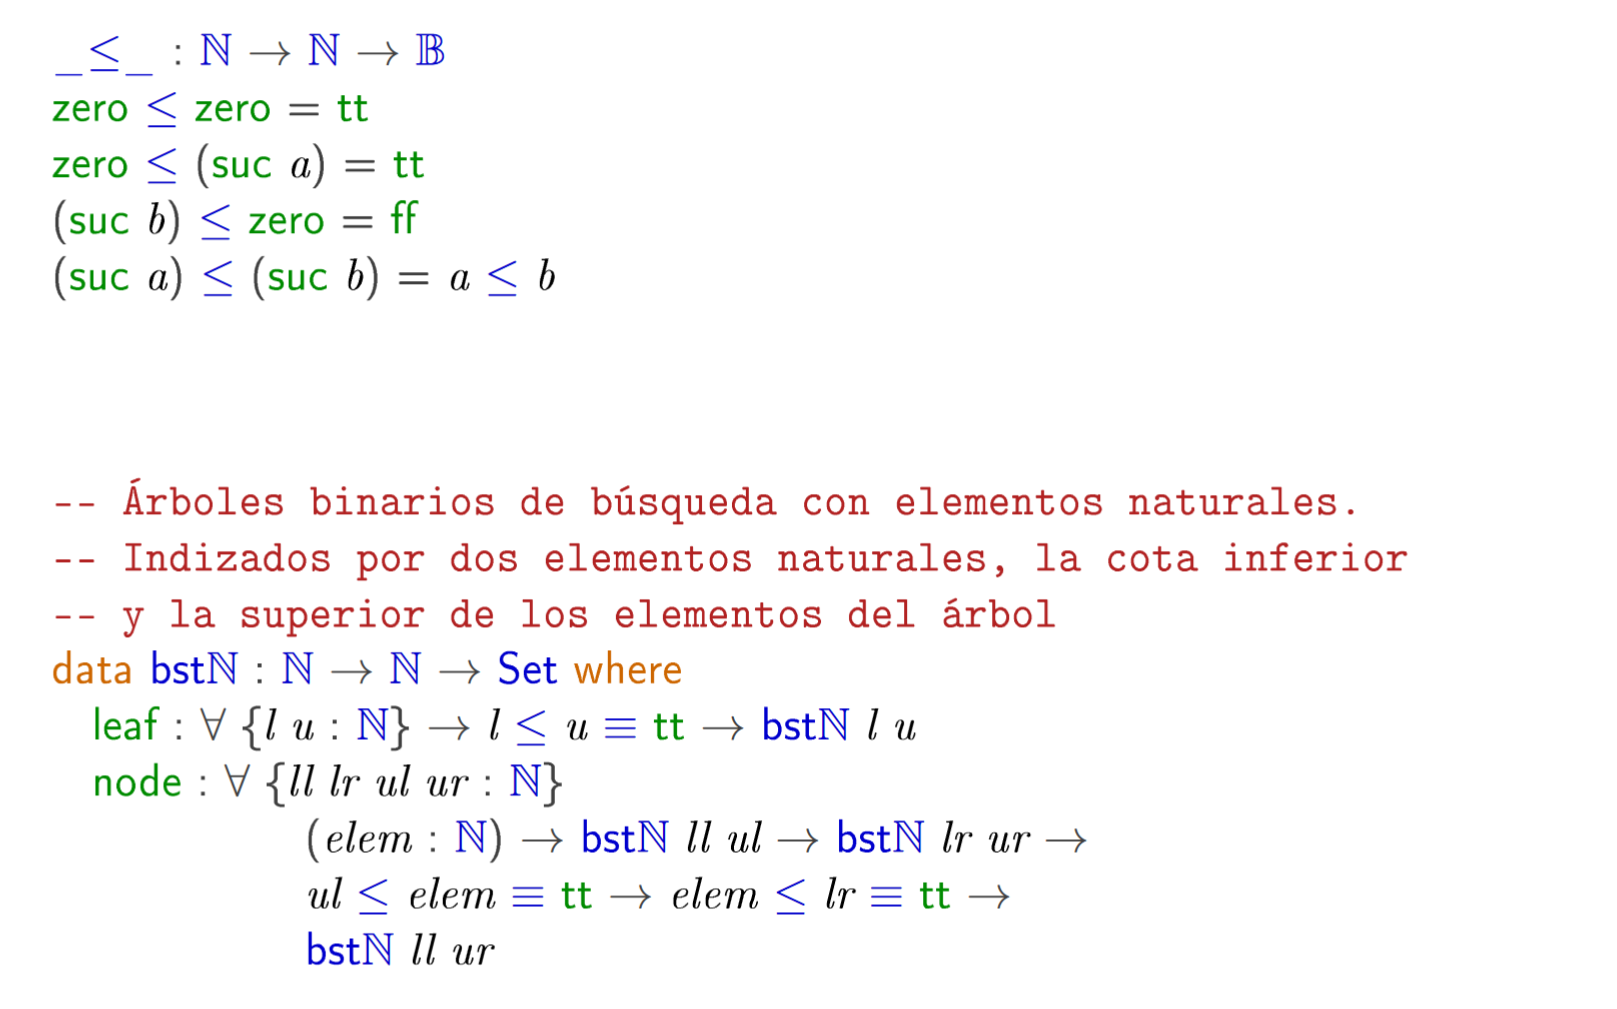
\includegraphics[scale=0.55]{img/bst}
\end{figure}

\end{frame}

\begin{frame}{Conclusiones}
\bit
\item Conclusiones respecto de Agda
\biti
\item Interesante e importante conocer el costado teórico
\item Experiencia interactiva muy rica
\item Intuitivo, estilo parecido a demostración en papel
\eit
\item Otras aproximaciones a la programación verificada
\biti
\item Coq
\item Haskell
\item Idris
\eit
\eit
\end{frame}

\end{document}
